% Options for packages loaded elsewhere
\PassOptionsToPackage{unicode}{hyperref}
\PassOptionsToPackage{hyphens}{url}
%
\documentclass[
  12 pt,
]{article}
\usepackage{amsmath,amssymb}
\usepackage{iftex}
\ifPDFTeX
  \usepackage[T1]{fontenc}
  \usepackage[utf8]{inputenc}
  \usepackage{textcomp} % provide euro and other symbols
\else % if luatex or xetex
  \usepackage{unicode-math} % this also loads fontspec
  \defaultfontfeatures{Scale=MatchLowercase}
  \defaultfontfeatures[\rmfamily]{Ligatures=TeX,Scale=1}
\fi
\usepackage{lmodern}
\ifPDFTeX\else
  % xetex/luatex font selection
\fi
% Use upquote if available, for straight quotes in verbatim environments
\IfFileExists{upquote.sty}{\usepackage{upquote}}{}
\IfFileExists{microtype.sty}{% use microtype if available
  \usepackage[]{microtype}
  \UseMicrotypeSet[protrusion]{basicmath} % disable protrusion for tt fonts
}{}
\makeatletter
\@ifundefined{KOMAClassName}{% if non-KOMA class
  \IfFileExists{parskip.sty}{%
    \usepackage{parskip}
  }{% else
    \setlength{\parindent}{0pt}
    \setlength{\parskip}{6pt plus 2pt minus 1pt}}
}{% if KOMA class
  \KOMAoptions{parskip=half}}
\makeatother
\usepackage{xcolor}
\usepackage[margin = 1.0in]{geometry}
\usepackage{longtable,booktabs,array}
\usepackage{calc} % for calculating minipage widths
% Correct order of tables after \paragraph or \subparagraph
\usepackage{etoolbox}
\makeatletter
\patchcmd\longtable{\par}{\if@noskipsec\mbox{}\fi\par}{}{}
\makeatother
% Allow footnotes in longtable head/foot
\IfFileExists{footnotehyper.sty}{\usepackage{footnotehyper}}{\usepackage{footnote}}
\makesavenoteenv{longtable}
\usepackage{graphicx}
\makeatletter
\def\maxwidth{\ifdim\Gin@nat@width>\linewidth\linewidth\else\Gin@nat@width\fi}
\def\maxheight{\ifdim\Gin@nat@height>\textheight\textheight\else\Gin@nat@height\fi}
\makeatother
% Scale images if necessary, so that they will not overflow the page
% margins by default, and it is still possible to overwrite the defaults
% using explicit options in \includegraphics[width, height, ...]{}
\setkeys{Gin}{width=\maxwidth,height=\maxheight,keepaspectratio}
% Set default figure placement to htbp
\makeatletter
\def\fps@figure{htbp}
\makeatother
\setlength{\emergencystretch}{3em} % prevent overfull lines
\providecommand{\tightlist}{%
  \setlength{\itemsep}{0pt}\setlength{\parskip}{0pt}}
\setcounter{secnumdepth}{-\maxdimen} % remove section numbering
\newlength{\cslhangindent}
\setlength{\cslhangindent}{1.5em}
\newlength{\csllabelwidth}
\setlength{\csllabelwidth}{3em}
\newlength{\cslentryspacingunit} % times entry-spacing
\setlength{\cslentryspacingunit}{\parskip}
\newenvironment{CSLReferences}[2] % #1 hanging-ident, #2 entry spacing
 {% don't indent paragraphs
  \setlength{\parindent}{0pt}
  % turn on hanging indent if param 1 is 1
  \ifodd #1
  \let\oldpar\par
  \def\par{\hangindent=\cslhangindent\oldpar}
  \fi
  % set entry spacing
  \setlength{\parskip}{#2\cslentryspacingunit}
 }%
 {}
\usepackage{calc}
\newcommand{\CSLBlock}[1]{#1\hfill\break}
\newcommand{\CSLLeftMargin}[1]{\parbox[t]{\csllabelwidth}{#1}}
\newcommand{\CSLRightInline}[1]{\parbox[t]{\linewidth - \csllabelwidth}{#1}\break}
\newcommand{\CSLIndent}[1]{\hspace{\cslhangindent}#1}
%%%%%%%%%%%%%%%%%%%%%%%%%%%%%%%%%%%%%%%%%%%%%%%%%%%%%%%%%%%%
% Font
%%%%%%%%%%%%%%%%%%%%%%%%%%%%%%%%%%%%%%%%%%%%%%%%%%%%%%%%%%%%

% Set font encoding to T1 (8-bit encoding, 256 glyphs) 
% (improved text handling, especially with non-English
% languages and text containing special characters)
\usepackage[T1]{fontenc}

% Set font to URW Nimbus Roman
% (Times New Roman alternative)
\usepackage{mathptmx}

%%%%%%%%%%%%%%%%%%%%%%%%%%%%%%%%%%%%%%%%%%%%%%%%%%%%%%%%%%%%
% Typsetting
%%%%%%%%%%%%%%%%%%%%%%%%%%%%%%%%%%%%%%%%%%%%%%%%%%%%%%%%%%%%

% Include the package containing commands for page orientation
\usepackage{pdflscape}
% Create a new custom command for starting a landscape block
\newcommand{\blandscape}{\begin{landscape}}
% Create a new custom command for ending a landscape block
\newcommand{\elandscape}{\end{landscape}}

% Include package providing fine-tuned typographic enhancements
\usepackage{microtype}

% Supress hyphenation
\usepackage[none]{hyphenat}

% Include package for setting spacing between lines
\usepackage{setspace}
% Set line spacing
\doublespacing

% Indent first paragraph of each section (including chapters)
\usepackage{indentfirst}

% Set vertical space between paragraphs
\setlength{\parskip}{1em}

%%%%%%%%%%%%%%%%%%%%%%%%%%%%%%%%%%%%%%%%%%%%%%%%%%%%%%%%%%%%
% Line numbers
%%%%%%%%%%%%%%%%%%%%%%%%%%%%%%%%%%%%%%%%%%%%%%%%%%%%%%%%%%%%

% Include package for line numbering
\usepackage{lineno}
% Set font style and size of line numbers
\renewcommand{\linenumberfont}{\normalfont\tiny}

%%%%%%%%%%%%%%%%%%%%%%%%%%%%%%%%%%%%%%%%%%%%%%%%%%%%%%%%%%%%
% Figures and tables
%%%%%%%%%%%%%%%%%%%%%%%%%%%%%%%%%%%%%%%%%%%%%%%%%%%%%%%%%%%%

% Include package enhancing figure and table placement
% (provides "H" placement specifier forcing the float to
% appear exactly where it is defined)
\usepackage{float}

% Include package used to create tables with cells spanning multiple rows
\usepackage{multirow}

%%%%%%%%%%%%%%%%%%%%%%%%%%%%%%%%%%%%%%%%%%%%%%%%%%%%%%%%%%%%
% Captions
%%%%%%%%%%%%%%%%%%%%%%%%%%%%%%%%%%%%%%%%%%%%%%%%%%%%%%%%%%%%

% Use a period as separator between the label and the caption text,
% and make the label bold
\usepackage[labelsep=space, labelfont=bf]{caption}
% Set caption text to be justified
\captionsetup{justification=justified}

%%%%%%%%%%%%%%%%%%%%%%%%%%%%%%%%%%%%%%%%%%%%%%%%%%%%%%%%%%%%
% Referencing
%%%%%%%%%%%%%%%%%%%%%%%%%%%%%%%%%%%%%%%%%%%%%%%%%%%%%%%%%%%%

% Include the package xr (external references) to allow
% referencing labels from another file
\usepackage{xr}
% Specify the name of the file used for additional
% referencing and define the prefix for the labels
% from the external document
\externaldocument[supp-]{supplementary}

%%%%%%%%%%%%%%%%%%%%%%%%%%%%%%%%%%%%%%%%%%%%%%%%%%%%%%%%%%%%
% Measurement units
%%%%%%%%%%%%%%%%%%%%%%%%%%%%%%%%%%%%%%%%%%%%%%%%%%%%%%%%%%%%

% Include the package that facilitates consistent formatting
% of scientific units and numbers
\usepackage{siunitx}
% Define unit \molar as moles per cubic decimeter
\DeclareSIUnit\molar{\mole\per\cubic\deci\metre}
% Define unit \Molar as small caps "M"  
\DeclareSIUnit\Molar{\textsc{m}}
% Define unit \cells as the text "cells"
\DeclareSIUnit\cells{\text{cells}}
% Define unit \litre as lowercase "l"
\DeclareSIUnit\litre{l}
% Define label \vV as v/v
\DeclareSIUnit{\vV}{v/v}
% Define label \wW as w/w
\DeclareSIUnit{\wW}{w/w}
% Define unit \bp as bp
\DeclareSIUnit{\bp}{bp}

%%%%%%%%%%%%%%%%%%%%%%%%%%%%%%%%%%%%%%%%%%%%%%%%%%%%%%%%%%%%
% Chemical formulae
%%%%%%%%%%%%%%%%%%%%%%%%%%%%%%%%%%%%%%%%%%%%%%%%%%%%%%%%%%%%

% Include package for typesetting chemical formulas
\usepackage{chemformula}
\ifLuaTeX
  \usepackage{selnolig}  % disable illegal ligatures
\fi
\IfFileExists{bookmark.sty}{\usepackage{bookmark}}{\usepackage{hyperref}}
\IfFileExists{xurl.sty}{\usepackage{xurl}}{} % add URL line breaks if available
\urlstyle{same}
\hypersetup{
  pdftitle={Influence of seagrass decline on the metabolic profile of sediment microbial communities},
  hidelinks,
  pdfcreator={LaTeX via pandoc}}

\title{\textbf{Influence of seagrass decline on the metabolic profile of sediment microbial communities}}
\author{}
\date{\vspace{-2.5em}}

\begin{document}
\maketitle

%%%%%%%%%%%%%%%%%%%%%%%%%%%%%%%%%%%%%%%%%%%%%%%%%%%%%%%%%%%%
% Captions
%%%%%%%%%%%%%%%%%%%%%%%%%%%%%%%%%%%%%%%%%%%%%%%%%%%%%%%%%%%%

% Set the name for figures to "Figure"
\renewcommand{\figurename}{Fig.}
% Use Arabic numerals to number figures
\renewcommand{\thefigure}{\arabic{figure}}

\vspace{\fill}

Marsej Markovski\textsuperscript{1}, Mirjana Najdek\textsuperscript{1}, Zihao Zhao\textsuperscript{2}, Gerhard J. Herndl\textsuperscript{2,3}, and Marino Korlević\textsuperscript{1*}

\begin{enumerate}
\def\labelenumi{\arabic{enumi}.}
\item
  Centre for Marine Research, Ruđer Bošković Institute, Croatia
\item
  Department of Functional and Evolutionary Ecology, University of Vienna, Austria
\item
  Department of Marine Microbiology and Biogeochemistry, Royal Netherlands Institute for Sea Research (NIOZ), Utrecht University, The Netherlands
\end{enumerate}

\textsuperscript{*}To whom correspondence should be addressed:

Marino Korlević

G. Paliaga 5, 52210 Rovinj, Croatia

Tel.: +385 52 804 768

e-mail: \href{mailto:marino.korlevic@irb.hr}{\nolinkurl{marino.korlevic@irb.hr}}

\linenumbers
\sisetup{mode=text}
\setlength\parindent{24pt}
\newpage

\hypertarget{abstract}{%
\section{Abstract}\label{abstract}}

{\setlength{\parskip}{0pt}

\noindent
\textbf{Background} Seagrass meadows are highly productive ecosystems that are considered hotspots for carbon sequestration. The decline of seagrass meadows of various species has been documented worldwide, including that of \emph{Cymodocea nodosa}, a widespread seagrass in the Mediterranean Sea. To assess the influence of seagrass decline on the metabolic profile of sediment microbial communities, metaproteomes from two sites, one without vegetation and one with a declining \emph{Cymodocea nodosa} meadow, were characterised at monthly intervals from July 2017 to October 2018.

\noindent
\textbf{Results} The differences in the metabolic profile observed between the vegetated and nonvegetated sediment before the decline were more pronounced in the deeper parts of the sediment and disappeared with the decay of the roots and rhizomes. During the decline, the protein richness and diversity of the metabolic profile of the microbial communities inhabiting the nonvegetated sediment became similar to those observed for the vegetated communities. Temporal shifts in the structure of the metabolic profile were only observed in the nonvegetated sediment and were also more pronounced in the deeper parts of the sediment. The assessment of the dynamics of proteins involved in the degradation of organic matter, such as ABC transporters, fermentation-mediating enzymes, and proteins involved in dissimilatory sulphate reduction, reflected the general dynamics of the metabolic profile.

\noindent
\textbf{Conclusions} Overall, the metabolic profile of the microbial communities inhabiting the nonvegetated sediment was influenced by the decline of seagrass, with stronger shifts observed in the deeper parts of the sediment.

}

\noindent
\textbf{Keywords} sediment microbial communities, \emph{Cymodocea nodosa}, seagrass meadow decline, northern Adriatic Sea, metaproteomics, microbial metabolic profile

\newpage

\hypertarget{background}{%
\section{Background}\label{background}}

Marine sediments cover around 70 \si{\percent} of the Earth's surface {[}1{]}. The biomass in these habitats consists mainly of prokaryotes, whose richness and abundance are comparable to that in the water column {[}1--3{]}. The main factor determining the abundance and activity of these microorganisms is the availability of organic matter {[}3--5{]}. Coastal waters supply large amounts of organic matter to the underlying sediments, which leads to the consumption of oxygen in the upper centimetres of the sediment and causes anoxic conditions in the deeper sediment {[}6{]}. The complete mineralisation of organic compounds in these anoxic environments requires complex microbial interactions {[}7--9{]}. The stepwise degradation of organic matter begins with the breakdown of complex organic polymers such as carbohydrates or proteins by extracellular enzymes that can be released into solution or remain associated with the cell. These enzymes convert high-molecular-weight organic matter to substrates that are small enough to be transported into the cell {[}10{]}. Part of these hydrolytic products are fermented to short-chain fatty acids (SCFAs) and alcohols that facilitate anaerobic microbial respiration, e.g.~by sulphate-reducing bacteria or methanogens {[}8, 9{]}.

Shallow coastal sediments colonised by seagrasses are considered a special type of habitat for marine prokaryotes {[}11{]}. Such areas are hotspots for microbial activity, as seagrasses enrich the sediment with organic matter by excreting organic carbon, trapping organic particles from the water column, and stabilising the sediment. In addition, the decomposition of seagrass leaves, roots, and rhizomes, which is particularly evident during the decline of the meadows, contributes to the enrichment of the sediment with organic matter {[}11--14{]}. Consequently, microbial communities in seagrass sediments are metabolically more diverse and active than those inhabiting bare sediments {[}15{]}. Furthermore, taxonomic analyses showed differences between communities at vegetated and nonvegetated sites {[}16--21{]} and indicated that microbial communities even differ with respect to the meadow edge {[}22{]}. The few available studies on microbial community succession in seagrass sediments suggest changes in sulphate-reducing bacteria over time {[}23{]}, as well as community changes in response to nutrient availability {[}24{]} and seagrass restoration {[}25{]}. However, there is not much information on the response of sediment microbial communities to seagrass decline. About 19 \si{\percent} of seagrass meadows worldwide have been lost since 1880 {[}26{]}. A decline of \emph{Cymodocea nodosa}, a widespread and common seagrass species throughout the Mediterranean Sea {[}27{]}, has been observed {[}28--31{]}, including in the northern Adriatic Sea {[}32--34{]}. In a previous study, we investigated the diversity and dynamics of sediment microbial communities during the decline of the seagrass species \emph{C. nodosa} and found a notable compositional stability in response to such a major disturbance {[}21{]}.

In order to obtain a comprehensive overview of the microbial communities living in sediments colonised by seagrasses, methods that allow functional characterisation, such as metaproteomics, must be applied. This high-throughput ``meta-omics'' approach is emerging as an important tool for deciphering the key components that determine the function of microbial ecosystems {[}35{]}. In addition, this approach has the potential to provide insights into the biogeochemical cycling in marine sediments and to assess the response of microbes to environmental change {[}36{]}. Metaproteomics is closely linked to metagenomics, as genome information in combination with data on expressed proteins not only provides information on the functional potential of microbial populations, but also on which metabolism is active in an ecosystem {[}37{]}. Metaproteomics has already been used to analyse microbial metabolic processes in cold seeps {[}38, 39{]}, diffuse hydrothermal venting {[}40{]}, mudflat aquaculture {[}41{]}, and chronically petroleum-polluted {[}42{]} sediments. To our knowledge there are no metaproteomic studies on microbial communities in seagrass meadow sediments. The aim of the present study was to use a metaproteomic approach to characterise the metabolic profile of prokaryotic communities in \emph{C. nodosa} meadow sediments and to determine the shifts in their metabolic profile when seagrass meadows decline.

\hypertarget{methods}{%
\section{Methods}\label{methods}}

\hypertarget{sampling}{%
\subsection{Sampling}\label{sampling}}

Sediment sampling for DNA and protein isolation was performed as described in Markovski et al.~(2022) {[}21{]}. For a detailed description of the sampling site, environmental conditions, and the decline of the \emph{C. nodosa} meadow, see Najdek et al.~(2020) {[}34{]}. In brief, sediment cores were collected from a declining \emph{C. nodosa} meadow (vegetated site) in the Bay of Saline (\ang{45;7;5} N, \ang{13;37;20} E) in the northern Adriatic Sea. An adjacent area without seagrass (nonvegetated site) was also sampled. Samples were taken monthly from July 2017 to October 2018. The meadow began to decline in November 2017, and by the end of the study, only small patches of seagrass along the shoreline indicated its former existence. Prior to DNA and protein isolation, the sediment cores were cut into four sections, each 1 cm long: the top (0 -- 1 cm), the bottom (7 -- 8 cm), and two middle sections: upper middle (2 -- 3 cm) and lower middle (3 -- 6 cm; Supplementary Table \ref{supp-tab:samples}).

\hypertarget{dna-isolation}{%
\subsection{DNA isolation}\label{dna-isolation}}

Total DNA from each sediment section was isolated using a modified isolation protocol {[}43{]} based on Zhou et al.~(1996) {[}44{]} as described in Markovski et al.~(2022) {[}21{]}. In brief, 2 \si{\gram} of sediment were weighed, avoiding roots and rhizomes in vegetated cores, mixed with the extraction buffer and proteinase K, and incubated by horizontal shaking at 37 \si{\degreeCelsius} for 30 \si{\minute}. After the addition of SDS, the mixture was incubated again by horizontal shaking at 65 \si{\degreeCelsius} for 60 \si{\minute}. The sediment particles were removed by centrifugation and the supernatant was extracted three times with an equal volume of chloroform:isoamyl alcohol (1:1). DNA precipitation was performed by adding isopropanol and incubating the mixture at 22 \si{\degreeCelsius} for 60 \si{\minute}. The DNA pellet obtained after the centrifugation step was washed twice with cold (\SI{-20}{\degreeCelsius}) 70 \si{\percent} ethanol, air-dried, and resuspended in 100 \si{\ul} of deionised water.

\hypertarget{metagenomics}{%
\subsection{Metagenomics}\label{metagenomics}}

Due to the limited number of sediment metagenomes that could have been sequenced, we selected four DNA samples from Markovski et al.~(2022) {[}21{]} collected in August 2018 from the top (0 -- 1 cm) and lower middle (4 -- 5 cm) layers of both the vegetated and nonvegetated sites (Supplementary Table \ref{supp-tab:metagenomes}). These selected DNA samples were sent on dry ice to IMGM Laboratories (Martinsried, Germany) for metagenomic sequencing. The genomic DNA was purified using AMPure XP Beads (Beckman Coulter, USA) at a bead:DNA ratio of 1:1 (\si{\vV}) and quantified using the Qubit dsDNA HS Assay Kit (Thermo Fisher Scientific, USA). The integrity of the DNA was checked on a 1 \si{\percent} agarose gel. Metagenomic sequencing libraries were prepared from 100 or 300 \si{\nano\gram} of genomic DNA using the NEBNext Ultra II FS DNA Library Prep Kit for Illumina (New England Biolabs, USA) according to the manufacturer's protocol. Fragments of 500 -- 700 \si{\bp} were selected using the AMPure XP Beads, enriched by PCR for 5 or 6 cycles, and quality controlled. The individual libraries generated from different DNA input samples were pooled and sequenced on an Illumina NovaSeq 6000 sequencing system (2 × 250 \si{\bp}).

The sequences obtained were analysed on the Life Science Compute Cluster (LiSC; CUBE -- Computational Systems Biology, University of Vienna). MEGAHIT (version 1.2.9) {[}45{]}, with default settings, was used to assemble individual metagenomic libraries and putative genes were predicted from contigs longer than 200 \si{\bp} using Prodigal (version 2.6.3) {[}46{]} in metagenome mode (-p meta). Predicted genes were functionally annotated using the eggNOG mapper (version 2.1.9) {[}47{]} with the eggNOG database (version 5.0.2) {[}48{]}. Taxonomic classification was performed using the lowest common ancestor algorithm from DIAMOND (version 2.0.15) {[}49{]} against the non-redundant NCBI database (NR). Phylogeny was determined using the top 10 \si{\percent} of hits with an e-value \textless{} 1 × 10\textsuperscript{-5} (-\/-top 10). Sequence renaming and the calculation of metagenomic statistics were performed using the tools from BBTools (\url{https://jgi.doe.gov/data-and-tools/bbtools}). In total, metagenomic sequencing generated between 205,085,833 and 216,556,629 sequence pairs (Supplementary Table \ref{supp-tab:metagenomes}). After the removal of low-quality reads, sequences were assembled into 21,634,340 to 33,248,196 contigs, with L50 ranging from 590 to 601 \si{\bp}. Coding sequence (CDS) prediction generated between 27,526,969 and 42,249,295 CDSs, while functional annotation resulted in 19,599,377 to 29,892,039 annotated CDSs.

\hypertarget{protein-isolation}{%
\subsection{Protein isolation}\label{protein-isolation}}

The proteins were isolated from the same sediment sections that were used for DNA isolation {[}21{]}. The SDS-based lysis method with trichloroacetic acid (TCA) precipitation described in Chourey et al.~(2010) {[}50{]} and modified by Hultman et al.~(2015) {[}51{]} was used. To 5 \si{\gram} of sediment, 10 \si{\percent} (\si{\wW}) polyvinylpolypyrolidone (PVPP) was added. The mixture was suspended in 5 \si{\ml} protein extraction buffer (4 \si{\percent} SDS and 100 \si{\milli\Molar} Tris-HCl {[}pH 8.0{]}) and vortexed. After incubation in boiling water for 5 \si{\minute}, the samples were sonicated and incubated again in boiling water for 5 \si{\minute}. Sonication was performed using the Sonopuls HD 4100 probe sonicator (Bandelin, Germany) equipped with an UW 100 ultrasonic transducer and a TS 103 probe. The solution was sonicated at 75 \si{\percent} of the maximum amplitude (245 \si{\um}) for 2 \si{\minute} at an interval of 10 \si{\s} on and 10 \si{\s} off. The sediment particles were removed by centrifugation for 20 \si{\minute} at 4 \si{\degreeCelsius} and 4,500 × \emph{g}. The supernatant was transferred to a clean tube and mixed with 1 \si{\Molar} dithiothreitol (DTT; final concentration 24 \si{\milli\Molar}). The proteins were precipitated with cold (\SI{4}{\degreeCelsius}) 100 \si{\percent} TCA (final concentration 20 \si{\percent}) overnight at \SI{-20}{\degreeCelsius}. The protein pellet was obtained by centrifugation for 40 \si{\minute} at 4 \si{\degreeCelsius} and 10,000 × \emph{g}. The obtained pellet was washed three times with cold (\SI{-20}{\degreeCelsius}) acetone and centrifuged after each washing step for 5 \si{\minute} at 4 \si{\degreeCelsius} and 20,000 × \emph{g}. The pellet was transferred to a clean 1.5 \si{\milli\liter} tube during the first washing step. The dried pellet was stored at \SI{-80}{\degreeCelsius} until further processing. In total, 120 protein samples were isolated.

\hypertarget{metaproteomics}{%
\subsection{Metaproteomics}\label{metaproteomics}}

The filter-aided sample preparation (FASP) {[}52{]} procedure was used to perform trypsin digestion. Isolated proteins were processed using the FASP Protein Digestion Kit (Expedeon, UK) according to the manufacturer's instructions, with minor modifications {[}53{]}. Briefly, the protein pellet was solubilised in the urea sample buffer included in the kit, amended with DTT, and centrifuged to remove larger particles. The trypsin digestion was performed on the column filter overnight at 37 \si{\degreeCelsius} for 18 \si{\hour}. The resulting filtrate containing peptides was acidified to a final concentration of 1 \si{\percent} trifluoroacetic acid (TFA). Digested peptides were desalted using the Pierce C18 Tips (Thermo Fisher Scientific, USA) according to the manufacturer's instructions and sent to the Proteomics Facilities of the University of Vienna for mass spectrometry analysis.

MS/MS spectra were obtained using a Q Exactive Hybrid Quadrupole-Orbitrap Mass Spectrometer (Thermo Fisher Scientific, USA) and searched against a protein database containing amino acid sequences of predicted CDSs from combined metagenomes that were sequenced and analysed as described above. MS/MS spectra were successfully generated for 118 samples (Supplementary Table \ref{supp-tab:samples}). Before the protein database search, the predicted CDSs were clustered at 90 \si{\percent} similarity using CD-HIT (version 4.6.8). Peptides were identified using the SEQUEST-HT engine and validated with Percolator, all within Proteome Discoverer (version 2.1; Thermo Fisher Scientific, USA). The probability of false peptide identification was reduced by applying the target-decoy approach. Only peptides with a false discovery rate \textless{} 1 \si{\percent} were retained. Protein identification required at least two peptides, including one unique peptide. Quantification of the relative abundance of proteins was conducted using a chromatographic peak area-based label-free quantitative method {[}54, 55{]}, where the peak areas of unique peptides were summed and normalised to the normalised area abundance factor (NAAF). In total, 67,947 different proteins were identified from the obtained MS/MS spectra. Of all identified proteins, 94.6 \si{\percent} were annotated by the eggNOG database. To focus exclusively on microbial communities, only proteins classified as \emph{Archaea} and \emph{Bacteria} using the NCBI database were retained. As a precautionary measure, proteins that were not taxonomically classified as \emph{Archaea} or \emph{Bacteria} by the eggNOG database were also removed, leaving a total of 57,305 proteins in the dataset.

\hypertarget{data-analysis}{%
\subsection{Data analysis}\label{data-analysis}}

Data processing and visualisation were performed using R (version 4.4.2) {[}56{]} combined with the tidyverse package (version 2.0.0) {[}57, 58{]} and several other packages {[}59--78{]}. The Shannon diversity index was calculated using the function \texttt{diversity} from the vegan package (version 2.6.4) {[}71{]}. To express the diversity index in terms of the effective number of proteins, the exponential of the Shannon diversity index was calculated {[}79{]}. Differences between the number of observed proteins, the exponential of the Shannon diversity index, and the NAAFs between sites, sediment layers, i.e., sections of sediment cores, and the period before and during the decay of \emph{C. nodosa} roots and rhizomes were tested by applying the Mann-Whitney \emph{U} test using the function \texttt{wilcox.test} {[}56{]}. The Bonferroni correction was applied to solve the problem of multiple comparisons using the function \texttt{p.adjust} {[}56{]}. Differences in the structure of the microbial metabolic profiles between sites, sediment layers, and the period before and during the decay of \emph{C. nodosa} roots and rhizomes were tested on Bray-Curtis dissimilarities based on protein NAAFs by performing the Analysis of Similarities (ANOSIM) using the function \texttt{anosim} from the vegan package and 999 permutations {[}71{]}. The grouping of samples into the period before and during the decay of roots and rhizomes was based on the decline of \emph{C. nodosa} reported by Najdek et al.~(2020) {[}34{]}. The sampling period from the beginning of the study until February 2018 was labelled the period before the decay of roots and rhizomes, while the period after this month was referred to as the period of decay of roots and rhizomes. Principal Coordinate Analysis (PCoA) was performed on Bray-Curtis dissimilarities based on protein NAAFs using the function \texttt{wcmdscale} from the vegan package. If necessary, the Lingoes correction method was applied to account for negative eigenvalues {[}71, 80, 81{]}.

\newpage

\hypertarget{results}{%
\section{Results}\label{results}}

To assess the richness and diversity of isolated proteins from the sediment microbial communities in the Bay of Saline, the number of observed proteins and the exponential of the Shannon diversity index were calculated. Samples from each layer were grouped based on the sampling site and the period before and during the decay of \emph{C. nodosa} roots and rhizomes. Comparisons between sampling sites in each period and between different periods at each site were performed (Fig. \ref{fig:alpha}). In all layers, significantly (\emph{p} \textless{} 0.05) higher numbers of observed proteins were found during the period before the decay of roots and rhizomes at the vegetated (top, 35,626 -- 37,937 proteins; upper middle, 32,494 -- 39,996 proteins; lower middle, 35,220 -- 39,713 proteins; and bottom, 32,183 -- 37,440 proteins) compared to the nonvegetated (top, 29,217 -- 36,284 proteins; upper middle, 29,312 -- 36,755 proteins; lower middle, 25,752 -- 33,630 proteins; and bottom, 27,672 -- 33,922 proteins) site. In contrast, no significant changes between sites were observed in all layers during the period of roots and rhizomes decay. In addition, no significant changes were found at each site between the two periods. When analysing the exponential of the Shannon diversity index, significant changes were observed only in the lower middle and bottom layer (Fig. \ref{fig:alpha}). Here, in agreement with the number of observed proteins, higher values were found during the period before the decay of roots and rhizomes at the vegetated (lower middle 7,594.2 -- 11,300.0 proteins and bottom, 3,927.3 -- 10,300.9 proteins) compared to the nonvegetated site (lower middle 1,497.2 -- 3,070.7 proteins and bottom, 586.6 -- 2,696.5 proteins). Also, in agreement with the number of observed proteins, no significant changes were observed between the sites during the period of roots and rhizomes decay. Additionally, the Shannon diversity index showed significant changes in these layers between the two periods. In the lower middle layer of the vegetated site, significantly higher values were observed before (7,594.2 -- 11,300.0 proteins) than during (4,254.3 -- 9,227.5 proteins) roots and rhizomes decay. However, in the bottom layer of the nonvegetated site significantly higher values were found during the period of roots and rhizomes decay (1,815.8 -- 6,775.9 proteins) than before the decay (586.6 -- 2,696.5 proteins).



\begin{figure}[H]

{\centering 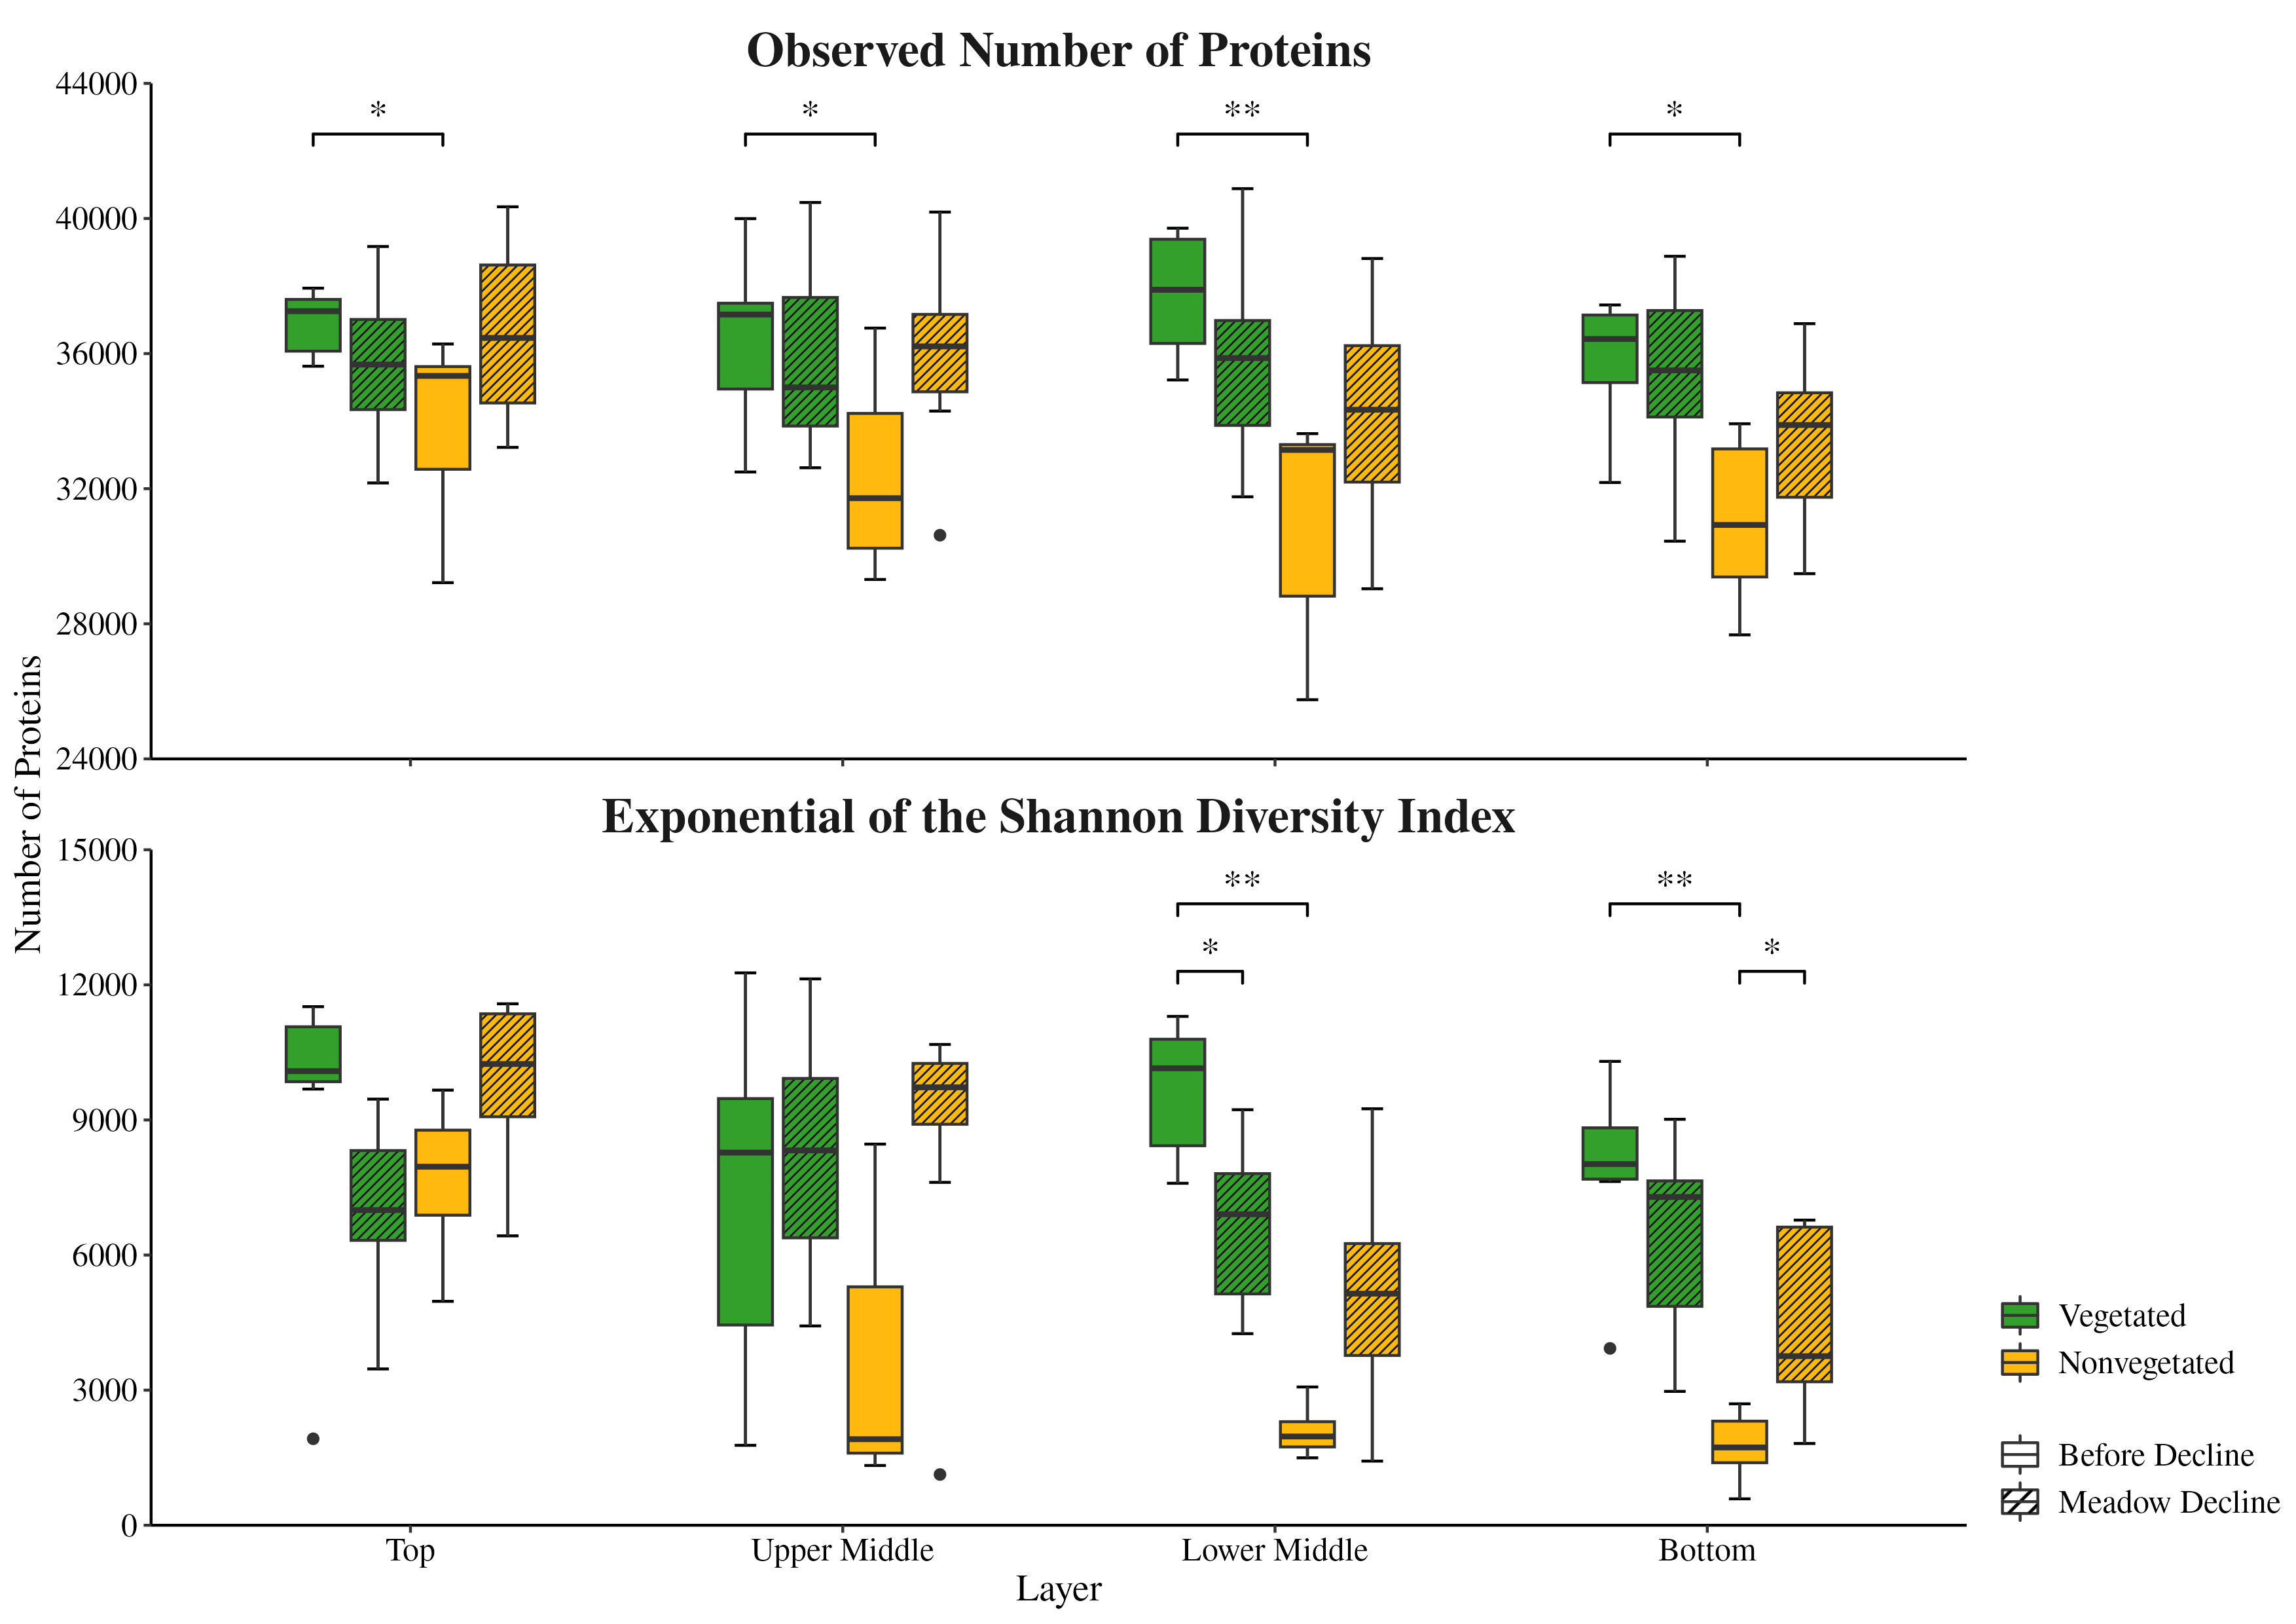
\includegraphics[width=1\linewidth]{../results/figures/alpha} 

}

\caption{The observed number of proteins and the exponential of the Shannon diversity index of sediment microbial communities in the Bay of Saline. Samples were collected in different sediment layers at the vegetated and nonvegetated site before and during the decay of roots and rhizomes of \emph{C. nodosa}. Asterisks indicate the level of statistical significance: \textbf{*}\emph{p} \textless{} 0.05 and \textbf{**}\emph{p} \textless{} 0.01.}\label{fig:alpha}
\end{figure}

ANOSIM testing of Bray-Curtis dissimilarities was applied to determine the changes in the structure of the metabolic profile of the sediment microbial communities. When all proteins from all samples were analysed together, no strong differentiation was observed between sites, layers, or the period before and during the decay of roots and rhizomes (ANOSIM, R = 0.14 -- 0.24, all \emph{p} \textless{} 0.01). To determine whether only a part of the metabolic network showed any differentiation, proteins classified in the Cluster of Orthologous Genes (COG) category C (energy production and conversion), the most abundant category in our samples (see below, Supplementary Table \ref{supp-tab:cog}), were analysed separately. However, no strong differentiation was observed between sites, layers, or decay periods when only these proteins were considered (ANOSIM, R = 0.15 -- 0.21, all \emph{p} \textless{} 0.01). In addition, the separate analysis of samples from the vegetated and nonvegetated site of all and COG C categorised proteins did also not reveal a strong differentiation between layers or decay periods (ANOSIM, R = 0.09 -- 0.26, all \emph{p} \textless{} 0.01), with the exception of a more pronounced separation observed at the nonvegetated site between the periods before and during the decay of roots and rhizomes. This separation could be observed when all proteins (ANOSIM, R = 0.33, \emph{p} \textless{} 0.01) and, especially, when proteins from the functional COG category C (ANOSIM, R = 0.51, \emph{p} \textless{} 0.01) were considered. To gain a clearer overview of this separation, samples from the nonvegetated site were analysed using PCoA (Fig. \ref{fig:pcoa-nonvegetated}). A distinction of samples from the lower middle and bottom layer retrieved during the period before the decay of roots and rhizomes from all other samples was noticed. This distinction could be observed when all proteins were analysed together, but especially when proteins from the functional COG category C were considered (Fig. \ref{fig:pcoa-nonvegetated}). Furthermore, to gain a better insight in the change of the structure of the metabolic profile between the period before and during the decay of roots and rhizomes, samples from each site and layer were analysed separately. Sediment layers of the vegetated site did not show any strong differentiation between these two periods when either all (ANOSIM, R = 0.05 -- 0.31, \emph{p} = 0.01 -- 0.23) or only COG C categorised proteins (ANOSIM, R = 0.12 -- 0.30, \emph{p} = 0.01 -- 0.05) were considered. In contrast, a pronounced separation between the two periods was observed in different layers of the nonvegetated site (Fig. \ref{fig:pcoa-layer}). When comparing the layers of this site, the lowest distinction between the two periods was observed in the top layer (ANOSIM; all proteins, R = 0.35, \emph{p} \textless{} 0.01; COG C proteins, R = 0.38, \emph{p} \textless{} 0.01), middle in the upper and lower middle layer (ANOSIM; all proteins, R = 0.29 -- 0.45, all \emph{p} \textless{} 0.01; COG C proteins, R = 0.53 -- 0.62, all \emph{p} \textless{} 0.01), and the highest in the bottom layer (ANOSIM; all proteins, R = 0.53, \emph{p} \textless{} 0.01; COG C proteins, R = 0.95, \emph{p} \textless{} 0.01).



\begin{figure}[H]

{\centering 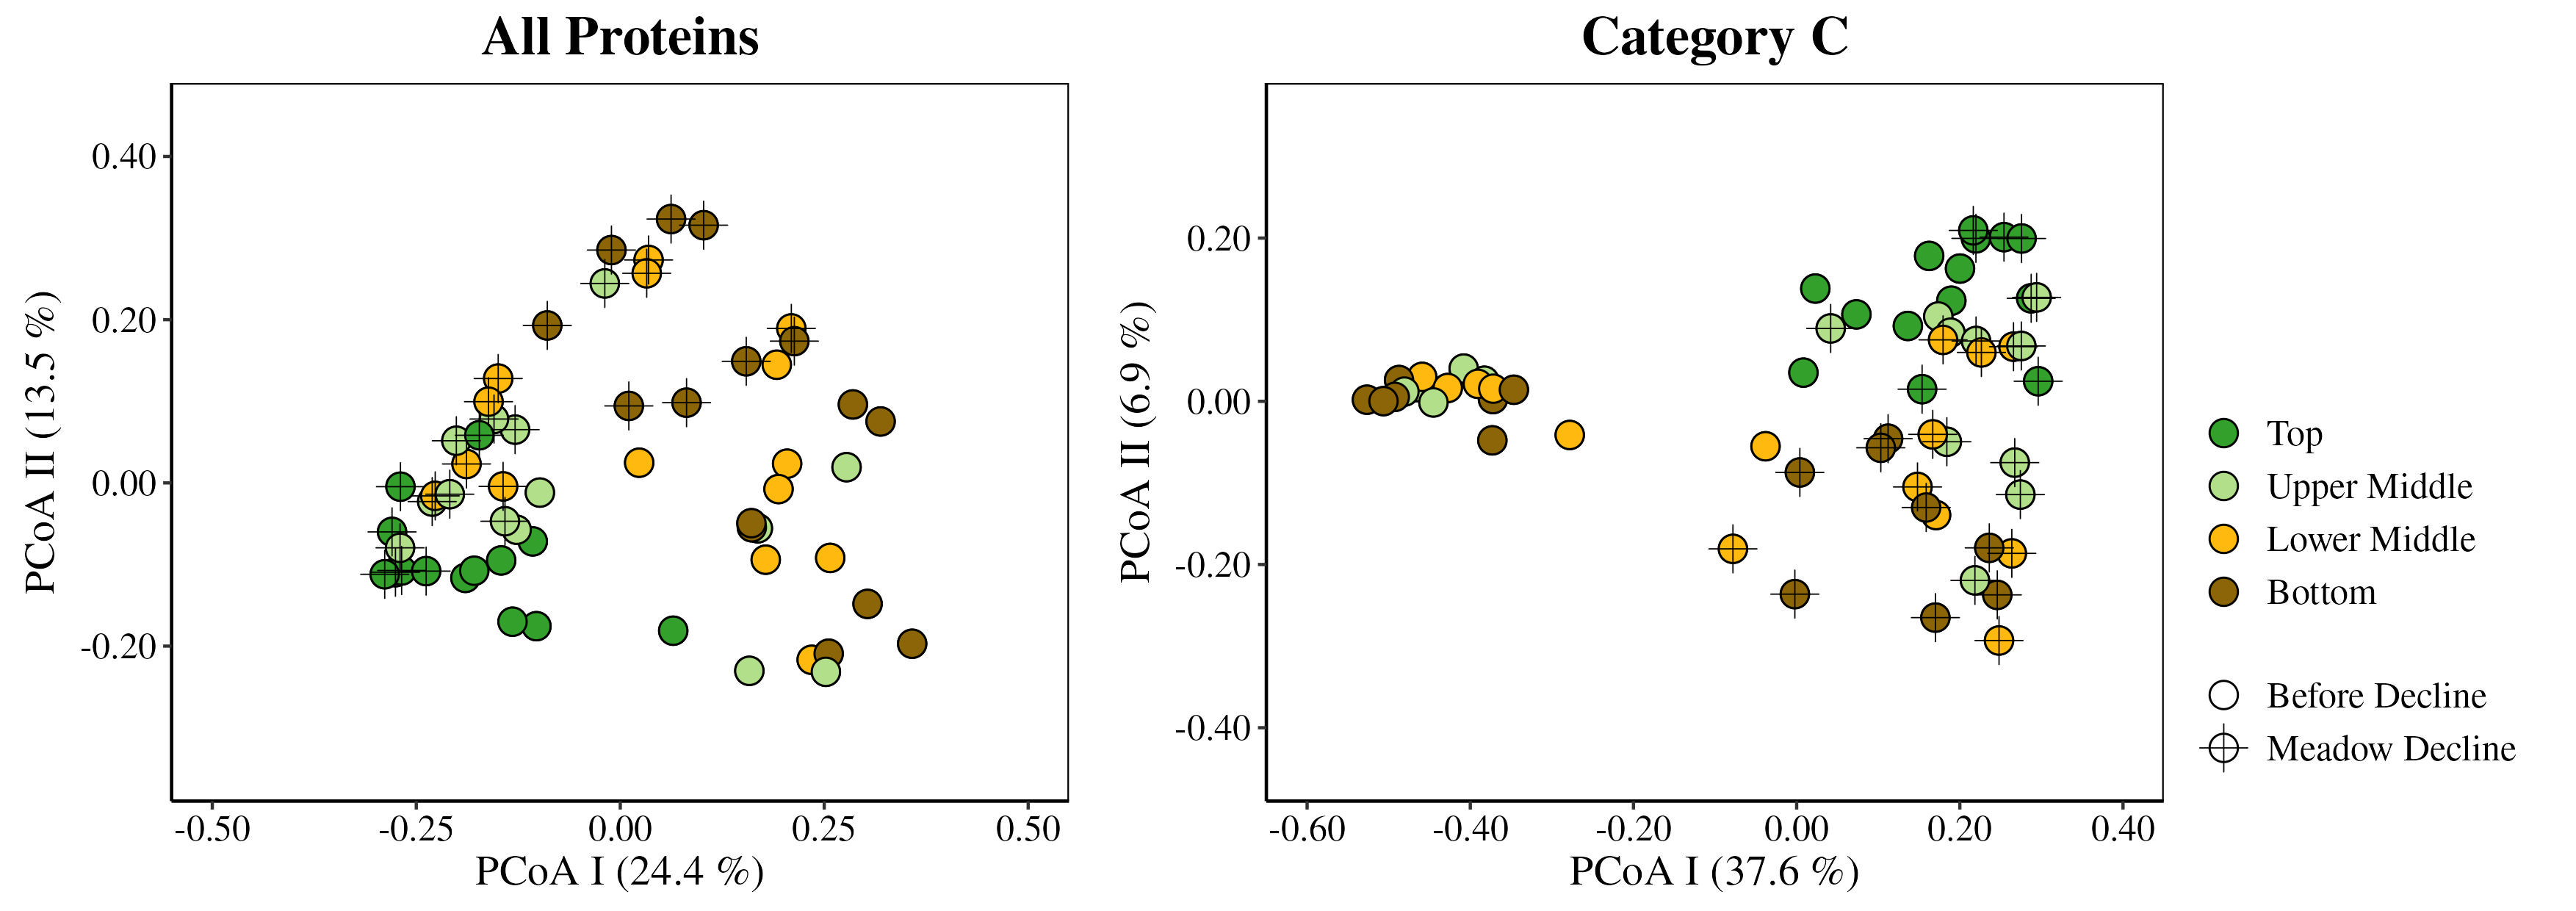
\includegraphics[width=1\linewidth]{../results/figures/pcoa_nonvegetated} 

}

\caption{PCoA of Bray-Curtis dissimilarities of microbial proteins sampled in the sediment of the Bay of Saline. All proteins and proteins classified only into COG category C (energy production and conversion) were analysed. Only samples collected in sediment layers at the nonvegetated site before and during decay of roots and rhizomes of \emph{C. nodosa} are shown. The proportion of variation explained by each axis is indicated in parentheses on the corresponding axis.}\label{fig:pcoa-nonvegetated}
\end{figure}

A total of 52,270 different proteins were assigned to a COG functional category. The most abundant COG category in terms of the number of proteins it contained (8,224 proteins) and their NAAFs (15.2 \si{\percent}) was the functional COG category C, which comprises proteins for energy production and conversion (Supplementary Table \ref{supp-tab:cog}). To detect how the decay of the meadow affected the energy production and conversion of sediment microbial communities in the Bay of Saline, we assessed the NAAF dynamics of the functional COG category C in each sediment layer. When comparing the sites before the decay of roots and rhizomes, significant (\emph{p} \textless{} 0.05) differences were only observed in the bottom layer where the proteins of this functional category comprised a larger proportion at the nonvegetated (19.5 -- 31.7 \si{\percent}) than at the vegetated (13.8 -- 26.2 \si{\percent}) site. No significant difference was found between the sites during the decay period. When comparing the layers of the individual sites before and during the decay of roots and rhizomes, we detected a significant change in the proportion of the functional COG category C only in the bottom layer of the nonvegetated site. Here, a significant decrease in the proportion of this functional category was observed between the period before (19.5 -- 31.7 \si{\percent}) and during (8.2 -- 13.9 \si{\percent}) the decay of roots and rhizomes.



\begin{figure}[H]

{\centering 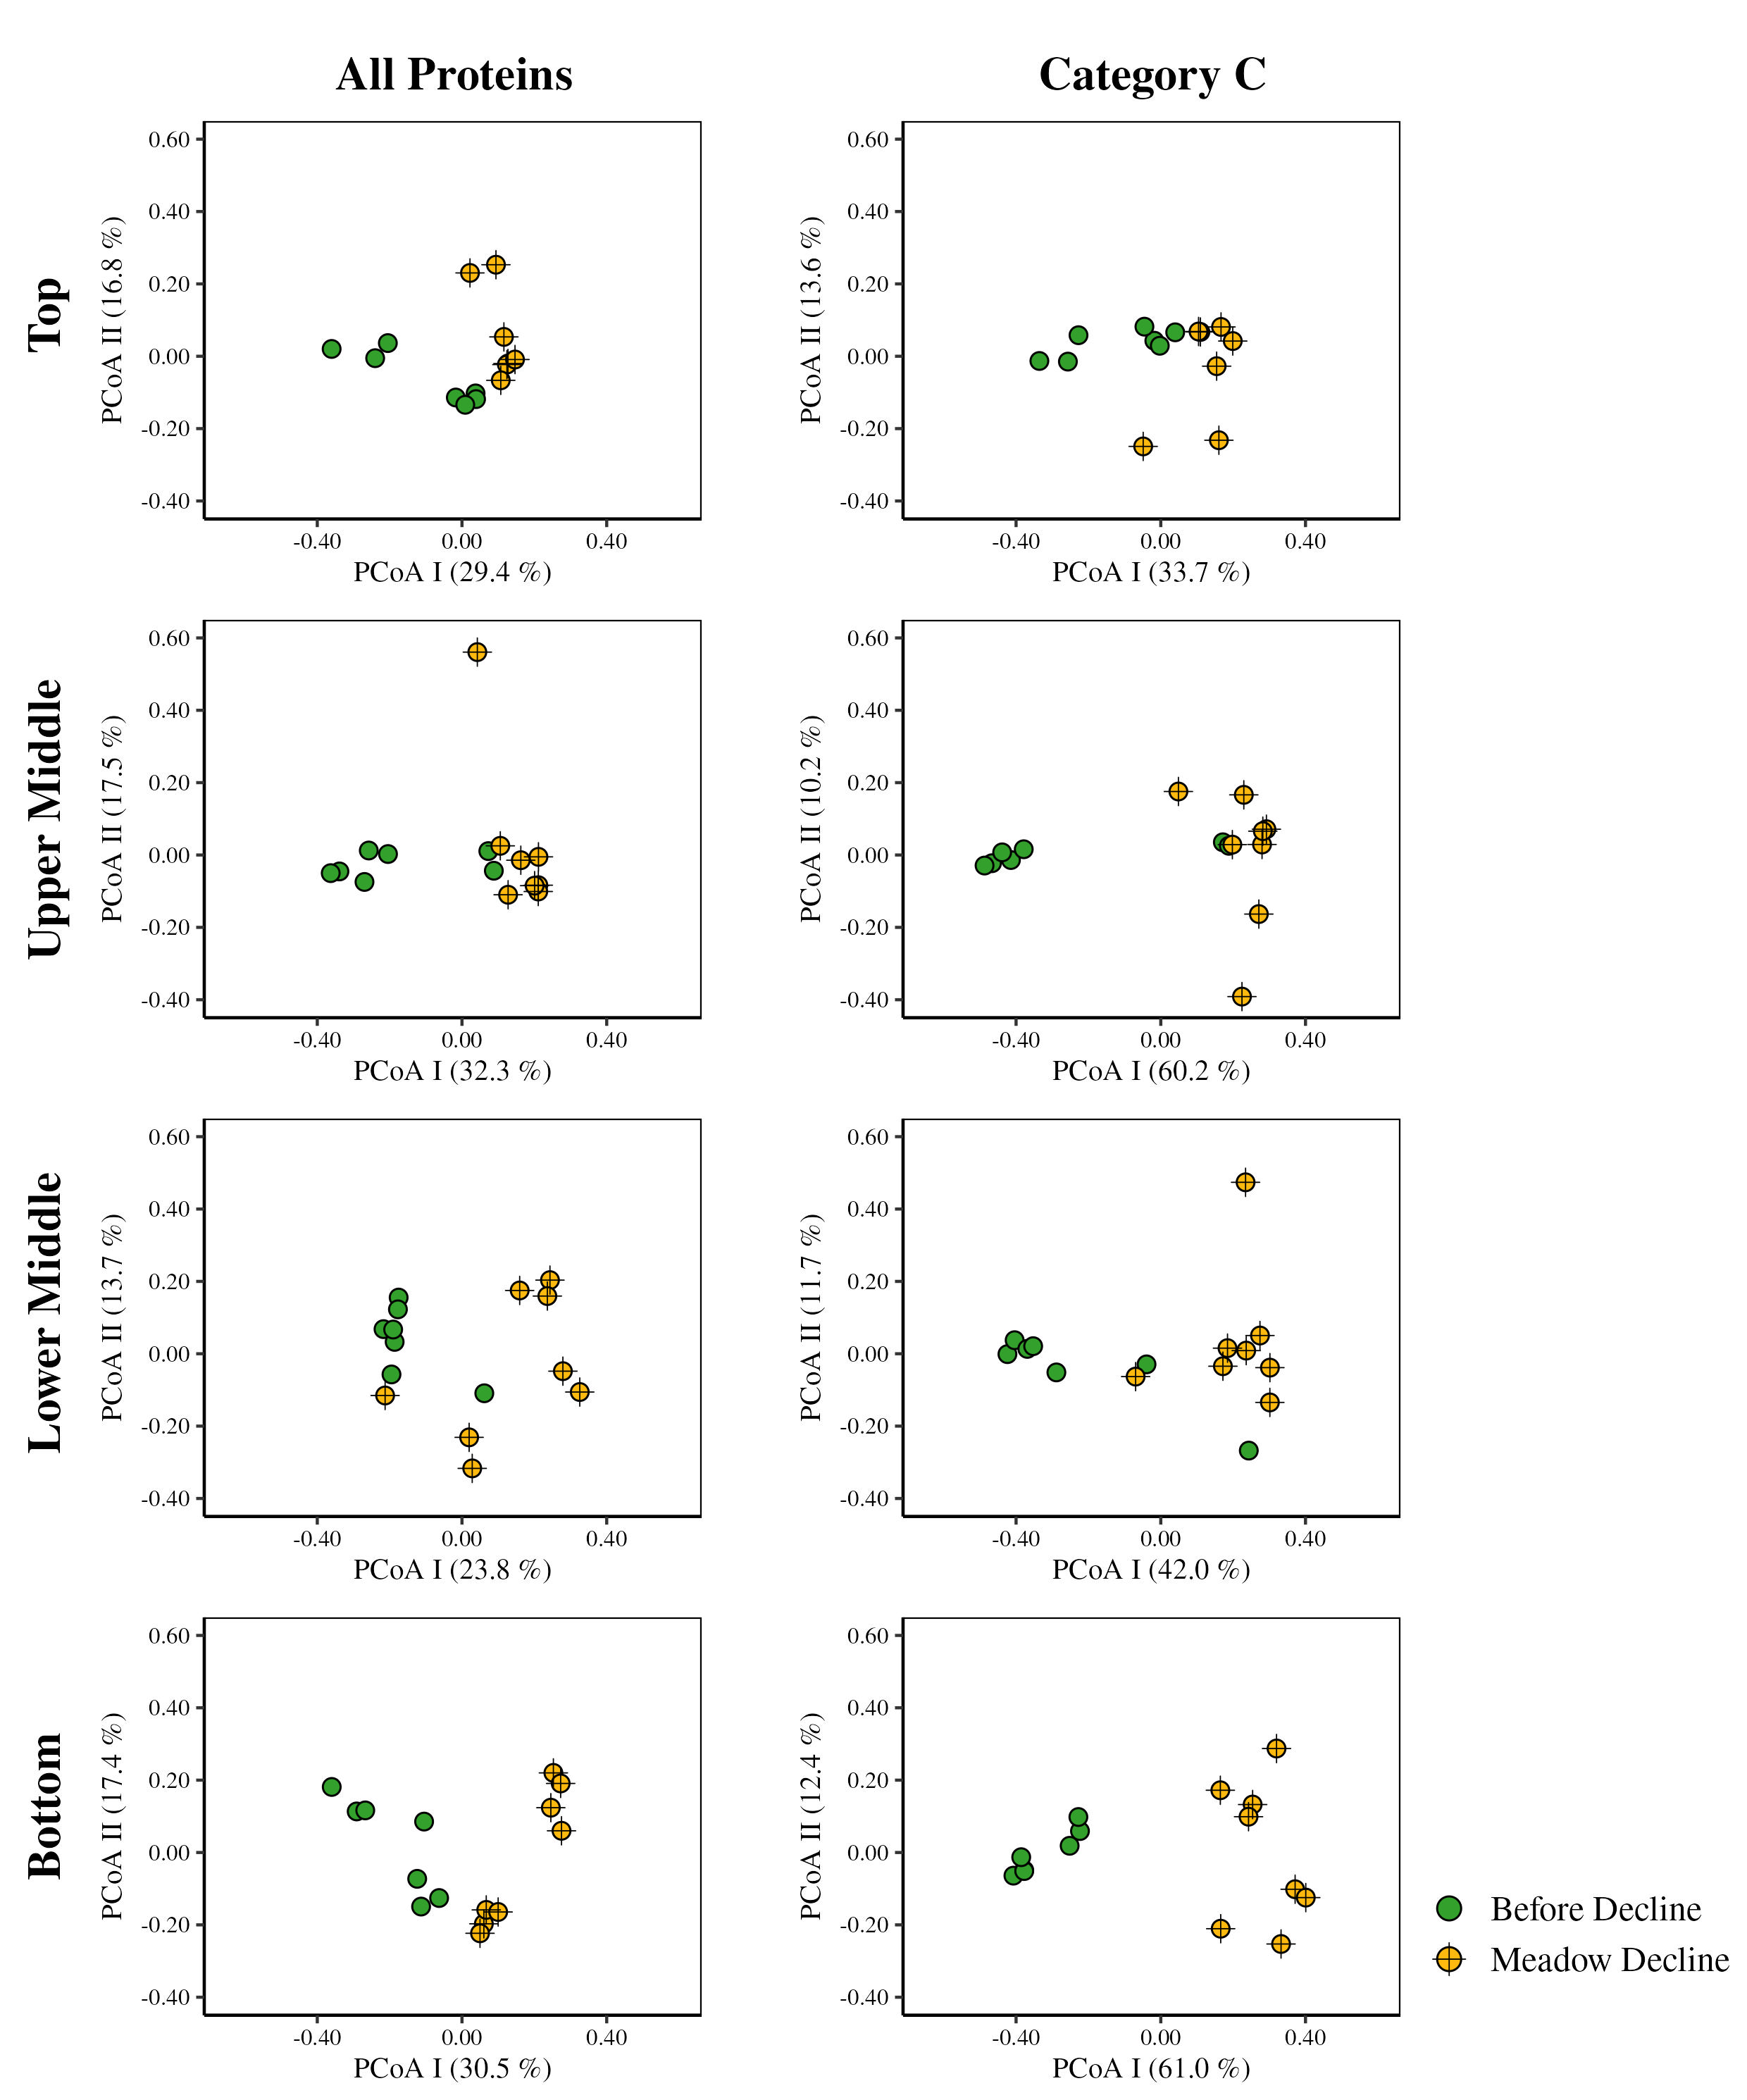
\includegraphics[width=0.95\linewidth]{../results/figures/pcoa_layer} 

}

\caption{PCoA of Bray-Curtis dissimilarities of microbial proteins sampled in each layer in the sediment of the Bay of Saline. All proteins and proteins classified only into COG category C (energy production and conversion) were analysed. Only samples collected at the nonvegetated site before and during decay of roots and rhizomes of \emph{C. nodosa} are shown. The proportion of variation explained by each axis is indicated in parentheses on the corresponding axis.}\label{fig:pcoa-layer}
\end{figure}

As the COG categories provide only a broad overview, the predicted CDSs were also classified using the Kyoto Encyclopaedia of Genes and Genomes (KEGG) Orthology (KO) database to gain better insight into the metabolic profile. A total of 1,408 different KO entries were present in the dataset, while 37,243 proteins were assigned to one or more of these KO entries. As the functional COG category C was the most abundant in our dataset (Supplementary Table \ref{supp-tab:cog}), we aimed to further explore the dynamics of the most pronounced KO entries within this category. The F-type H\textsuperscript{+}-transporting ATPase subunit c (ATPF0C, atpE; 20.0 \si{\percent}), the K\textsuperscript{+}-stimulated pyrophosphate-energized sodium pump (hppA; 7.9 \si{\percent}), and the adenylylsulphate reductase subunits A (aprA; 6.2 \si{\percent}) and B (aprB; 6.1 \si{\percent}) represented the highest proportion (NAAF) within the functional COG category C (Fig. \ref{fig:cog-c-kegg}). As the samples from the nonvegetated site showed a clear separation based on the period of roots and rhizomes decay, especially when the COG category C dataset was considered (Fig. \ref{fig:pcoa-nonvegetated}), we compared the proportion of these three proteins at the nonvegetated site before and during the decay of roots and rhizomes (Fig. \ref{fig:cog-c-kegg}). We observed a significant (\emph{p} \textless{} 0.05) decrease in the proportion of the F-type H\textsuperscript{+}-transporting ATPase subunit c during the decay of roots and rhizomes in all layers. This decrease was particularly pronounced in the bottom layer, where this protein constituted between 52.7 and 76.0 \si{\percent} of all COG C categorised proteins before the decay. During the decay of roots and rhizomes, its proportion dropped to between 3.2 and 19.3 \si{\percent}. Although not as pronounced as the change in the F-type H\textsuperscript{+}-transporting ATPase subunit c, the K\textsuperscript{+}-stimulated pyrophosphate-energized sodium pump also showed a significant shift between the two periods in all layers, except the top layer. The most significant shift was observed in the bottom layer, where this protein increased from between 0.8 and 4.9 \si{\percent} of all COG categorised proteins before the decay to between 4.9 and 11.6 \si{\percent} during the decay (\emph{p} \textless{} 0.001). The proportion of the adenylylsulphate reductase subunits A and B also increased during the decay in all layers, with the exception of the top layer. However, this shift was only significant in the bottom layer, where this protein increased from 3.5 to 7.4 \si{\percent} of all COG categorised proteins before the decay to 12.1 to 15.7 \si{\percent} during the decay.



\begin{figure}[H]

{\centering 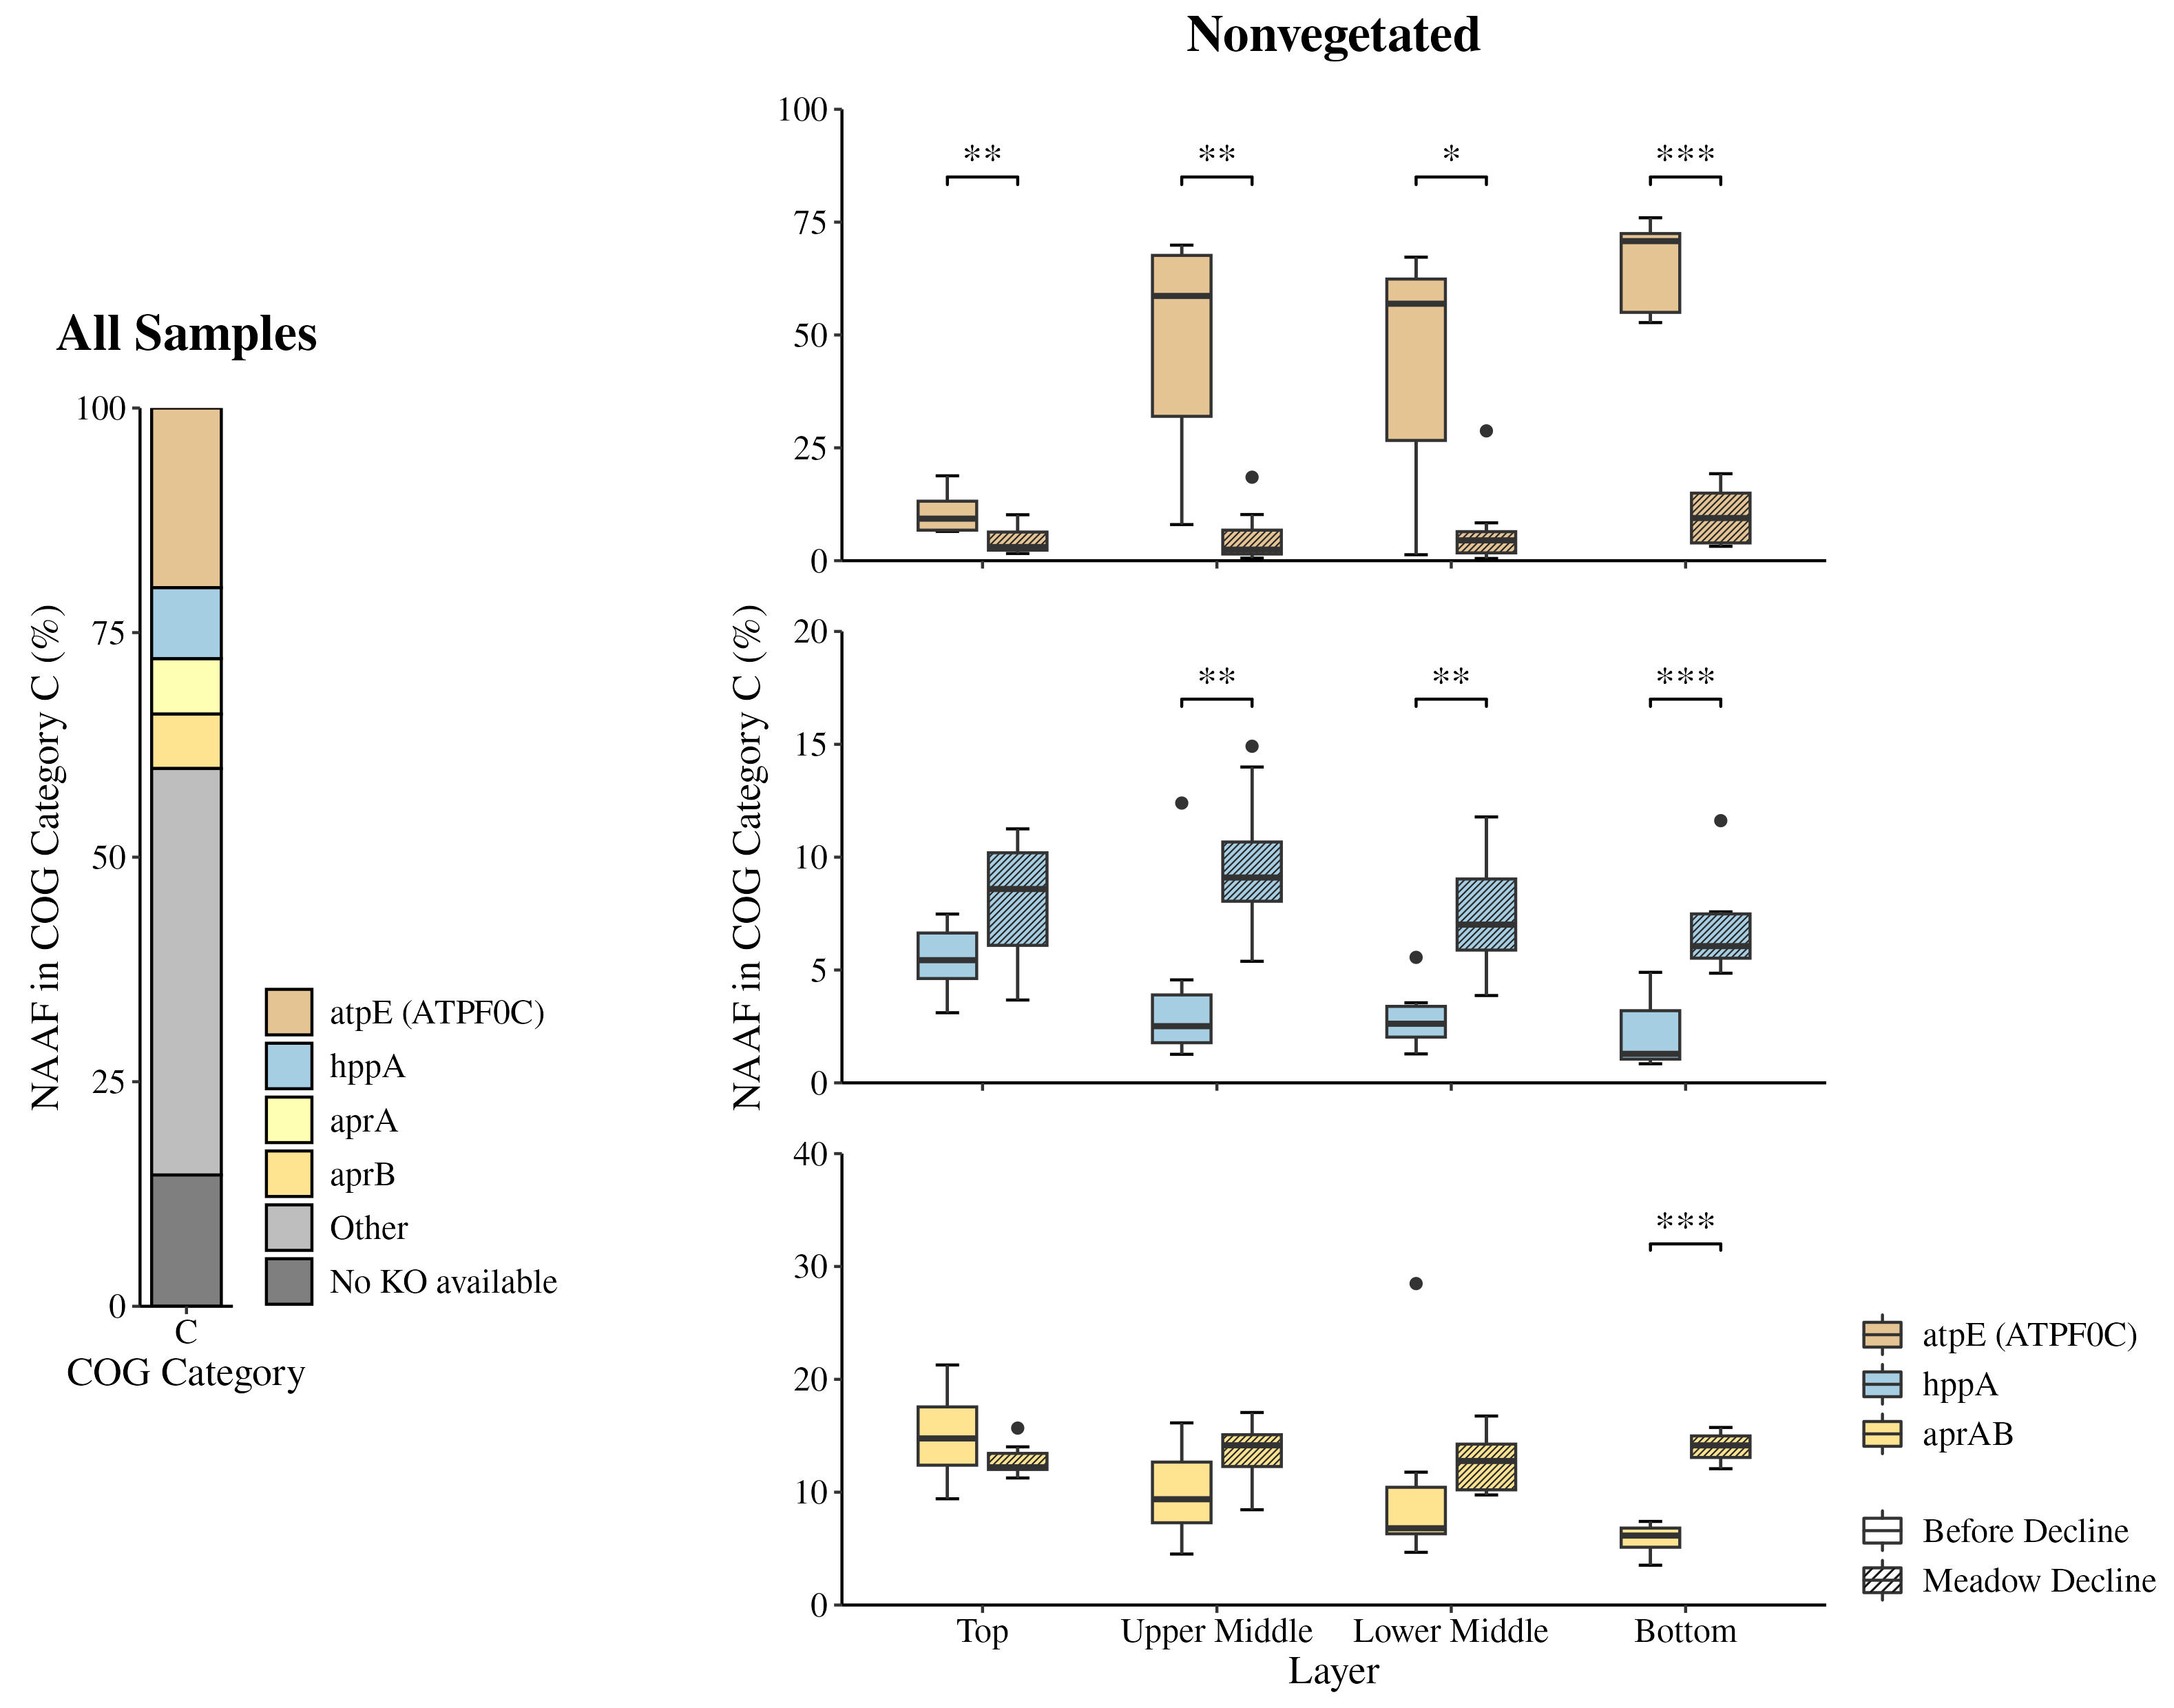
\includegraphics[width=1\linewidth]{../results/figures/cog_c_kegg} 

}

\caption{Proportion of the most abundant (\textgreater{} 3 \si{\percent}) KEGG KO entries within the functional COG category C (energy production and conversion) in all samples and changes in the proportion of the same entries in each layer at the nonvegetated site before and during the decay of roots and rhizomes of \emph{C. nodosa} in the Bay of Saline. The proportion was calculated using the NAAF. Asterisks indicate the level of statistical significance: \textbf{*}\emph{p} \textless{} 0.05, \textbf{**}\emph{p} \textless{} 0.01, and \textbf{***}\emph{p} \textless{} 0.001.}\label{fig:cog-c-kegg}
\end{figure}

The degradation of complex organic matter by the sediment microbial community in the Bay of Saline was evaluated by assessing the dynamics of the carbohydrate, protein, and lipid hydrolytic enzymes (Fig. \ref{fig:heatmap-hydrolases-abc-transporters}). The dynamics of carbohydrate hydrolytic enzymes was determined using Carbohydrate-Active enZymes (CAZymes), whose proportion did not significantly (\emph{p} \textless{} 0.05) change between stations or decay periods, with the exception of the top sediment layer at the nonvegetated site. Here, a significant decrease in the proportion of CAZymes was observed from the period before decay (0.28 -- 0.43 \si{\percent}) to the period of roots and rhizomes decay (0.22 -- 0.28 \si{\percent}; Fig. \ref{fig:heatmap-hydrolases-abc-transporters}). Proteins assigned to the glycoside hydrolase families GH5 and GH9 were the most abundant of all CAZymes (47.2 \si{\percent}). To assess protein degradation, we focused on proteins assigned as peptidases in KEGG. The proportion of these enzymes significantly increased in the upper middle layer of the vegetated site from the period before decay (0.15 -- 0.45 \si{\percent}) to the period of roots and rhizomes decay (0.34 -- 0.61 \si{\percent}; Fig. \ref{fig:heatmap-hydrolases-abc-transporters}). Peptidases were almost exclusively comprised of metalloendopeptidases and serine endopeptidases (93.3 \si{\percent}). Compared to CAZymes and peptidases, lipases were the least represented in our data (Fig. \ref{fig:heatmap-hydrolases-abc-transporters}).

We assessed the dynamics of ATP-binding cassette (ABC) transporters to evaluate the uptake of hydrolytic products by prokaryotic cells. Substrate-binding proteins classified as ABC transporters in the KEGG Pathway (map02010) were selected and further manually classified into the following categories based on the molecules they transport: sugar, peptide, amino acid, urea, lipid, polyol, phosphate, and mineral and organic ion (Fig. \ref{fig:heatmap-hydrolases-abc-transporters}). Sugar (38.0 \si{\percent}) and amino acid (31.5 \si{\percent}) transporters were the most abundant among all selected ABC transporters. In the lower middle and bottom layer, a significantly (\emph{p} \textless{} 0.05) higher proportion of sugar ABC transporters was observed at the vegetated (lower middle, 2.90 -- 4.57 \si{\percent}; bottom, 3.90 -- 5.52 \si{\percent}) than at the nonvegetated (lower middle, 2.25 -- 3.20 \si{\percent}; bottom, 1.75 -- 2.81 \si{\percent}) site during the period before roots and rhizomes decay (Fig. \ref{fig:heatmap-hydrolases-abc-transporters}). In contrast, no significant differences in the proportion of ABC transporters targeting sugars between sites were observed during the period of roots and rhizomes decay. These transporters also showed a significant increase in the bottom layer of the nonvegetated site from the period before decay (1.75 -- 2.81 \si{\percent}) to the period of roots and rhizomes decay (2.16 -- 6.79 \si{\percent}). The proportion of ABC transporters targeting amino acids only showed a significant increase in the bottom layer of the nonvegetated site from the period before decay (2.05 -- 3.02 \si{\percent}) to the period of roots and rhizomes decay (2.76 -- 4.62 \si{\percent}).



\begin{figure}[H]

{\centering 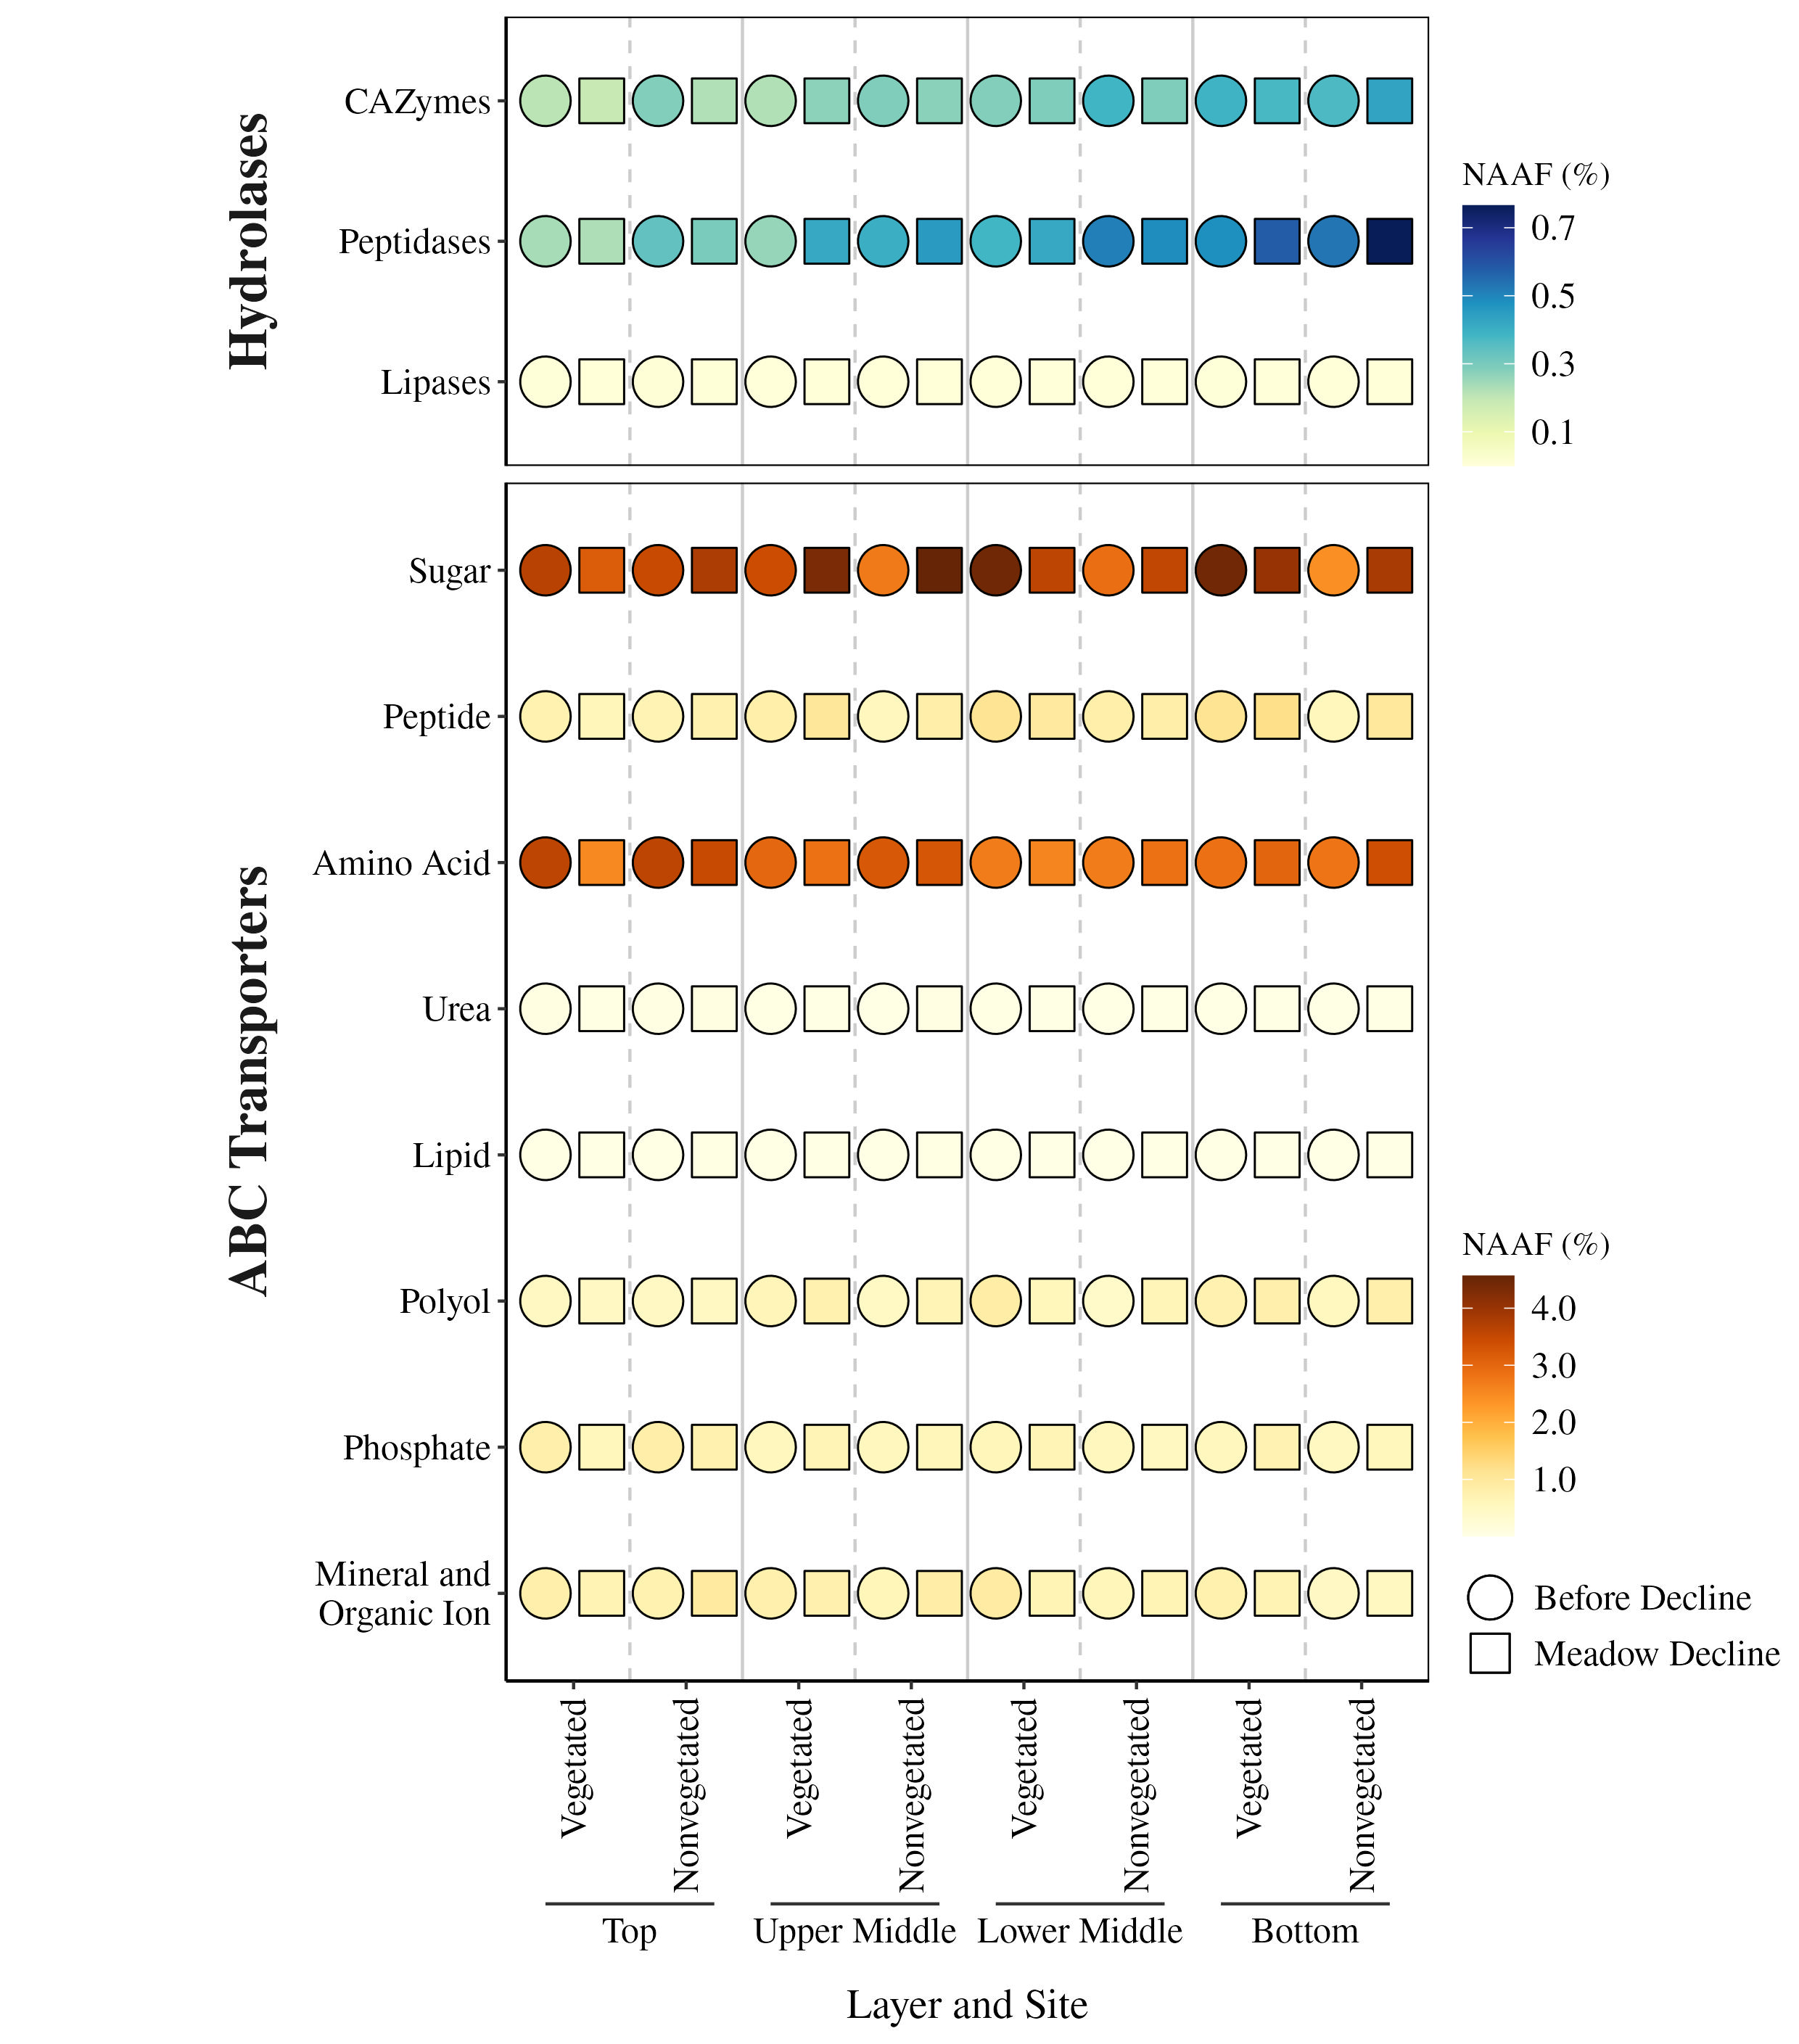
\includegraphics[width=0.9\linewidth]{../results/figures/heatmap_hydrolases_abc_transporters} 

}

\caption{Median proportion of groups of hydrolases and ABC transporters in sediment layers at the vegetated and nonvegetated site before and during the decay of roots and rhizomes of \emph{C. nodosa} in the Bay of Saline. The proportion was calculated using the NAAF.}\label{fig:heatmap-hydrolases-abc-transporters}
\end{figure}

To evaluate the role of fermentation processes at these two sites, we selected enzymes from the KEGG database that are thought to be involved in mediating various fermentation products such as carbon dioxide, formate, acetate, acetone, ethanol, lactate, acetoin, propionate, and butyrate (Supplementary Table \ref{supp-tab:fermentation}). Of these selected enzymes, our dataset contained pyruvate:ferredoxin oxidoreductase, pyruvate formate-lyase, acetyl-CoA hydrolase, acetate kinase, and alcohol, formate, and lactate dehydrogenase (Fig. \ref{fig:heatmap-fermentation-dsr}). Formate dehydrogenase (45.2 \si{\percent}), pyruvate:ferredoxin oxidoreductase (31.4 \si{\percent}), and alcohol dehydrogenase (17.0 \si{\percent}) were the most prominent of all fermentation-mediating enzymes detected. Significantly (\emph{p} \textless{} 0.05) higher proportions of formate dehydrogenase were detected before the decay of roots and rhizomes in the lower middle layer of the vegetated (0.28 -- 0.45 \si{\percent}) compared to the nonvegetated (0.20 -- 0.30 \si{\percent}) site. In contrast, no significant differences were observed during the decay of roots and rhizomes. A similar trend was observed for pyruvate:ferredoxin oxidoreductase in the bottom layer, which had a higher proportion of this enzyme before the decay of roots and rhizomes at the vegetated (0.14 -- 0.30 \si{\percent}) compared to the nonvegetated (0.09 -- 0.22 \si{\percent}) site. However, no significant differences between sites were observed during the decay of roots and rhizomes (Fig. \ref{fig:heatmap-fermentation-dsr}). Alcohol dehydrogenase showed significant differences between sites in both the lower middle and bottom layer. In the lower middle layer, a higher proportion of this enzyme was observed at the vegetated than at the nonvegetated site before (vegetated, 0.08 -- 0.16 \si{\percent}; nonvegetated; 0.04 -- 0.07 \si{\percent}) and during the decay of roots and rhizomes (vegetated, 0.07 -- 0.43 \si{\percent}; nonvegetated; 0.04 -- 0.11 \si{\percent}). The same pattern of higher proportions of this enzyme at the vegetated site before (vegetated, 0.08 -- 0.26 \si{\percent}; nonvegetated; 0.05 -- 0.07 \si{\percent}) and during roots and rhizomes decay (vegetated, 0.13 -- 0.88 \si{\percent}; nonvegetated; 0.06 -- 0.14 \si{\percent}) was also detected in the bottom layer.

To obtain an overview of the different microbial metabolic processes occurring in the sediment of the Bay of Saline, we selected KEGG modules describing methane-, nitrogen-, and sulphur-related processes (Supplementary Table \ref{supp-tab:metabolism}). Among all tested modules we found proteins involved in the following processes: methanogenesis, nitrogen fixation, dissimilatory nitrate reduction, denitrification, assimilatory and dissimilatory sulphate reduction, and thiosulphate oxidation by the SOX complex. Since one of the most prominent proteins in the functional COG category C (energy production and conversion) was the adenylylsulphate reductase (Fig. \ref{fig:cog-c-kegg}), which is involved in dissimilatory sulphate reduction, the dynamics of the enzymes involved in this process were investigated in more detail. Of the enzymes involved in dissimilatory sulphate reduction, our dataset contained sulphate adenylyltransferase, adenylylsulphate reductase, and dissimilatory sulphite reductase (Fig. \ref{fig:heatmap-fermentation-dsr}). The proportion of adenylylsulphate reductase was much higher (75.0 \si{\percent}) than that of sulphate adenylyltransferase (11.1 \si{\percent}) and dissimilatory sulphite reductase (13.9 \si{\percent}). Significantly (\emph{p} \textless{} 0.05) higher proportions of sulphate adenylyltransferase were observed before roots and rhizomes decay at the vegetated than at the nonvegetated site in the upper middle (vegetated, 0.18 -- 0.55 \si{\percent}; nonvegetated, 0.10 -- 0.28 \si{\percent}), lower middle (vegetated, 0.27 -- 0.61 \si{\percent}; nonvegetated, 0.06 -- 0.19 \si{\percent}), and bottom (vegetated, 0.17 -- 0.32 \si{\percent}; nonvegetated, 0.06 -- 0.20 \si{\percent}) layer. In addition, significantly higher proportions were also found in the bottom layer of the nonvegetated site during roots and rhizomes decay (0.14 -- 0.35 \si{\percent}) compared to the period before the decay (0.06 -- 0.20 \si{\percent}). Proportions of the adenylylsulphate reductase showed significant changes in the lower middle layer, where higher values were observed before roots and rhizomes decay at the vegetated (1.99 -- 3.05 \si{\percent}) compared to the nonvegetated (1.22 -- 2.53 \si{\percent}) site. Also, in the same layer of the vegetated site significantly higher proportions were detected before roots and rhizomes decay (1.99 -- 3.05 \si{\percent}) compared to the period of the decay (1.33 -- 2.40 \si{\percent}). In the lower middle and bottom layer, dissimilatory sulphite reductase showed higher proportions before roots and rhizomes decay at the vegetated (lower middle, 0.37 -- 0.78 \si{\percent}; bottom, 0.25 -- 0.42 \si{\percent}) than at the novegetated (lower middle, 0.16 -- 0.40 \si{\percent}; bottom, 0.11 -- 0.21 \si{\percent}) site. In addition, significantly higher proportions were detected in the bottom layer of the nonvegetated site during roots and rhizomes decay (0.17 -- 0.39 \si{\percent}) compared to the period before the decay (0.11 -- 0.21 \si{\percent}). In contrast, no significant differences between stations were observed during the decay of roots and rhizomes for either of these enzymes (Fig. \ref{fig:heatmap-fermentation-dsr}).



\begin{figure}[H]

{\centering 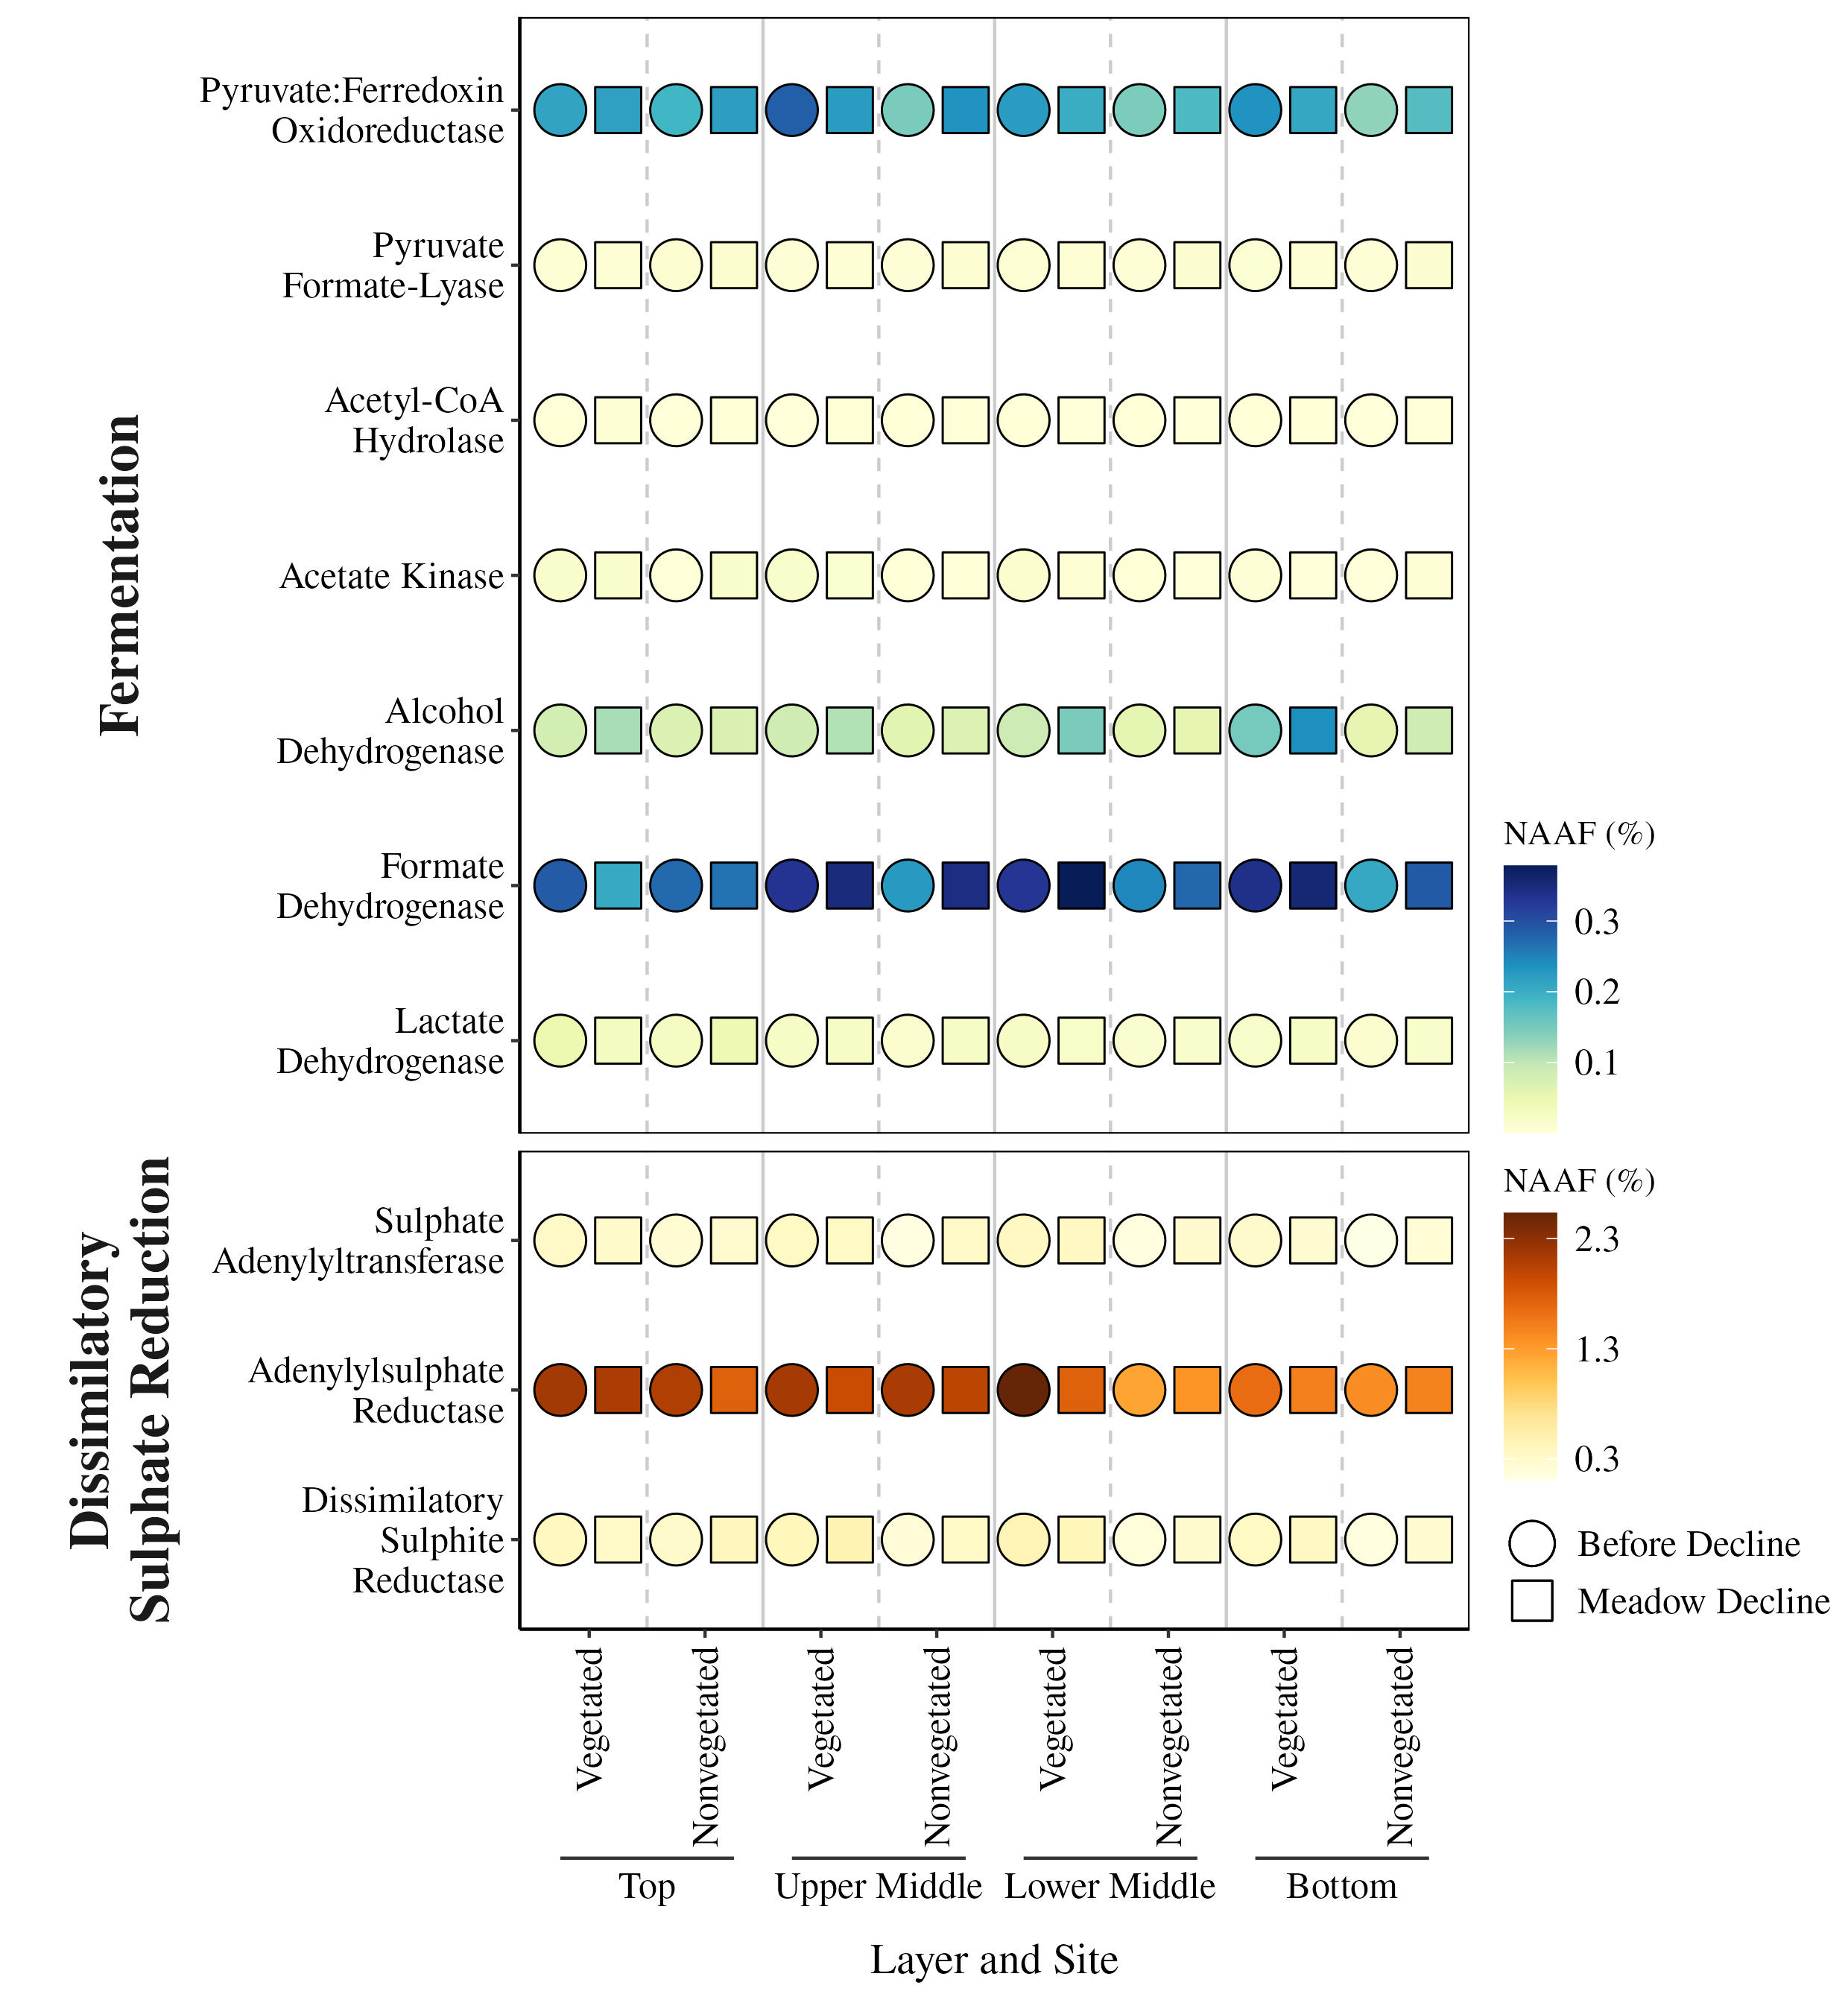
\includegraphics[width=0.9\linewidth]{../results/figures/heatmap_fermentation_dsr} 

}

\caption{Median proportion of enzymes involved in mediating various fermentation products and dissimilatory sulphate reduction in sediment layers at the vegetated and nonvegetated site before and during the decay of roots and rhizomes of \emph{C. nodosa} in the Bay of Saline. The proportion was calculated using the NAAF.}\label{fig:heatmap-fermentation-dsr}
\end{figure}

\newpage

\hypertarget{discussion}{%
\section{Discussion}\label{discussion}}

Seagrass meadow habitats are highly productive ecosystems {[}82{]} that support high biodiversity {[}83{]}. In the present study, before the decay of the roots and rhizomes of \emph{C. nodosa}, higher values of the number of observed proteins and of the exponential of the Shannon diversity index were found in the vegetated compared to the nonvegetated sediment. These differences were more pronounced in the deeper parts of the sediment (i.e., in the lower middle and bottom layer). After the decay, the differences began to disappear and the values of the number of observed proteins and of the Shannon diversity index were similar to those observed in the sediment previously inhabited by the meadow. In addition, the structure of the metabolic profile of the communities inhabiting the nonvegetated sediment showed a separation between the period before and during the decay of roots and rhizomes, especially in the deeper parts of the sediment and when only proteins for energy production and conversion were considered. This pattern was not observed for the communities at the vegetated site. The difference between the microbial communities inhabiting the vegetated and nonvegetated sediment in the period before roots and rhizomes decay is not surprising, as several studies have found that the presence of seagrass leads to the formation of sediment communities that differ in composition {[}16--22{]} and function {[}15{]} from communities inhabiting nonvegetated sediments. In addition, the higher values of the number of observed proteins and of the Shannon diversity index at the vegetated site before the decay are consistent with other studies reporting higher metabolic diversity and microbial community activity in seagrass sediments compared to nonvegetated areas and with higher organic matter content in seagrass-inhabited sediments {[}11, 15{]}. In addition, the greater differentiation observed in the deeper layers in terms of protein richness and diversity is consistent with a previous study on the same sediment communities, which found a greater community separation between sites in the deeper parts of the sediment {[}21{]}. In contrast, the less pronounced differentiation observed for the same parameters and for the structure of the metabolic profile in the top and upper middle layer could be explained by the input of organic matter derived from the vegetated site, making the communities in the upper part of the sediment more similar to each other. Indeed, organic matter imported from the seagrass meadow has been shown to be an important source for prokaryotes in nonvegetated sediments {[}84{]}.

The lack of differences between sites during the decay of roots and rhizomes in the number of observed proteins and in the exponential of the Shannon diversity index indicates the presence of a more uniform microbial metabolic profile during this period, similar to the metabolic profile observed at the vegetated site prior to decline. This observation is supported by the greater similarity in the structure of the metabolic profile of the communities at the nonvegetated site during decline with the metabolic profile of the communities in the upper sediment prior to decline. Because seagrass meadows fix the sediment by reducing resuspension rates and sediment mixing {[}85{]}, we hypothesise that resuspension, mixing, and transport between sites are enhanced when the meadow is no longer present, allowing greater input of fresh organic matter to the nonvegetated sediment. Indeed, Najdek et al.~(2020) {[}34{]} reported higher levels of total lipids and organic matter at the nonvegetated site during the \emph{C. nodosa} decline from May to August 2018. The uniformity of the microbial profile observed at the vegetated site during the study could be the result of maintaining the source of organic matter during the decline of the seagrass through the decay of leaves, roots, and rhizomes {[}11--14{]}.

The analysis of the functional COG categories showed that category C, which includes proteins for energy production and conversion, was the most abundant. This is consistent with the metagenomic study of Habibi et al.~(2023) {[}86{]}, who reported that energy production and conversion was also one of the most abundant functional COG categories in coastal sediments. Among these proteins, F-type H\textsuperscript{+}-transporting ATPase subunit c, K\textsuperscript{+}-stimulated pyrophosphate-energized sodium pump, and adenylylsulphate reductase subunits A and B exhibited the highest proportion. The pronounced presence of the F-type H\textsuperscript{+}-transporting ATPase subunit c in the deeper parts of the nonvegetated sediment prior to decay could be explained by the involvement of this enzyme in the generation of membrane potential. The F-type ATPase can work in both directions, utilising the proton gradient to generate ATP or hydrolysing the ATP to generate the membrane potential {[}87{]}. The high proportion of the K\textsuperscript{+}-stimulated pyrophosphate-energized sodium pump in our dataset indicates the coupling of the energy released by pyrophosphate hydrolysis with the active transport of cations across membranes {[}88, 89{]}. The proportion of this protein was increased in the deeper parts of the nonvegetated sediment during decay, reflecting the need of microbial communities for more active cross-membrane transport probably due to the increased input of fresh organic matter from the vegetated site. The high proportion of adenylylsulphate reductase subunits A and B among the proteins for energy production and conversion is not surprising, as this enzyme is part of dissimilatory sulphate reduction to sulphide, a predominant terminal pathway of organic matter mineralisation in anoxic seabeds, where it reduces adenosine-5\('\)-phosphosulphate to sulphite {[}90{]}. Furthermore, its significantly higher proportion in the nonvegetated sediment during decay could also be explained by the enhancement of this terminal pathway as a result of increased input of fresh organic matter from the vegetated site.

High molecular weight organic matter in marine sediments must be converted into low molecular weight molecules by various hydrolytic enzymes so that it can be taken up by cells {[}10{]}. Important components of organic matter in coastal marine sediments are carbohydrates, proteins, and lipids {[}91{]}. In our dataset, CAZymes and peptidases were more abundant than lipases, which may indicate the importance of carbohydrates and proteins as sources of organic matter for the microbial community. Among the CAZymes, the glycoside hydrolase families GH5 and GH9 were the most abundant. These families contain members capable of hydrolysing plant organic matter such as cellulose {[}92--94{]}. The presence of enzymes acting on cellulose is not surprising as cellulose is a major component of seagrass cell walls and contributes between 20 and 77 \si{\percent} to the dry plant material {[}95--97{]}. Metalloendopeptidases and serine endopeptidases made up the vast majority of peptidases in our dataset. A high proportion of these enzymes among the extracellular proteases has already been reported for coastal sediments {[}98--100{]}. CAZymes and peptidases showed no dynamics from pre-decay to decay of roots and rhizomes, except that CAZymes decreased in the top layer of the nonvegetated sediment and peptidases increased in the upper middle layer of the vegetated sediment. Studies have shown that the molar carbon:nitrogen content in seagrass litter decreases during the decomposition process, which could be explained by increased microbial colonisation of detrital matter and microbial utilisation of exogenous nitrogen which could be related to the observed decrease in CAZymes and increase in peptidases {[}12, 14{]}.

Once complex organic compounds have been broken down, the hydrolytic products can be transported into the cells. Prokaryotes utilise various transport proteins, including ABC transporters, to import substrates. Our metaproteomic dataset contained a large amount of ABC transporters for sugars and amino acids. Previous studies of sediment metagenomes also reported a high proportion of ABC transporters {[}86, 101{]}. The dynamics of ABC transporters reflected the overall dynamics of the metabolic profile. ABC transporters for sugars showed a higher proportion in the deeper parts of the vegetated compared to the nonvegetated sediment before decay of roots and rhizomes and showed no differences between sites during decay, reflecting the higher organic matter content and corresponding demand for ABC transporters in seagrass-inhabited sediments {[}11, 15{]}. In addition, ABC transporters for sugars and amino acids showed an increase in their proportion in the bottom layer of the nonvegetated sediment from the period before decay to the decay of the roots and rhizomes, which could be attributed to changes in organic matter content during the decline of the meadow.

The hydrolytic products of the degradation of complex organic matter, such as simple sugars and amino acids, can be imported and consumed by fermenting microbes. We have identified several enzymes involved in mediating various fermentation products, of which formate dehydrogenase, pyruvate:ferredoxin oxidoreductase, and alcohol dehydrogenase are the most abundant. Microcosm studies of the anaerobic degradation of organic matter in marine sediments revealed that acetate, formate, and ethanol are the most common fermentation products {[}102, 103{]}. In addition, direct measurements of sediment pore water have revealed the presence of methanol and ethanol {[}104{]}. It is therefore not surprising that the most common fermentation-mediating enzymes we found are putatively involved in the metabolism of acetate, formate, and ethanol. In addition, pyruvate:ferredoxin oxidoreductase and alcohol dehydrogenase have also been reported to be important fermentation-mediating enzymes in Baltic Sea sediments {[}105{]}. Similar to the dynamics of the ABC transporters, the fermentation-mediating enzymes also reflected the overall dynamics of the metabolic profile. Formate dehydrogenase, pyruvate:ferredoxin oxidoreductase, and alcohol dehydrogenase showed increased proportions in the deeper parts of the vegetated compared to the nonvegetated sediment before the decay of roots and rhizomes, reflecting the higher organic matter content and possibly a higher fermentation rate in seagrass-inhabited sediments {[}11, 15{]}.

The final step in the anaerobic degradation of organic matter involves the utilisation of simpler compounds such as SCFAs, including acetate and formate, and alcohols by the sulphate-reducing bacteria or methanogens {[}8, 9{]}. One of the most prominent proteins in functional COG category C was adenylylsulphate reductase, which is involved in dissimilatory sulphate reduction (Fig. \ref{fig:heatmap-fermentation-dsr}). Dissimilatory sulphate reduction is known to be a predominant terminal pathway of organic matter mineralisation in anoxic seabeds {[}90{]}. Sulphate adenylyltransferase (Sat), adenylylsulphate reductase (Apr), and dissimilatory sulphite reductase (Dsr), enzymes involved in the dissimilatory sulphate reduction pathway shared by known sulphate-reducing microorganisms {[}90{]}, were also detected in our metaproteomic dataset. The dynamics of these enzymes showed some common patterns that were comparable to the overall dynamics of the metabolic profile. Overall, higher proportions of these enzymes were found in the deeper parts of the vegetated compared to the nonvegetated site before roots and rhizomes decay, while such differences were not present during decay. This pattern as well as the overall dynamics of the metabolic profile could be explained by the higher organic matter content in the seagrass-inhabited sediments before decay {[}11, 15{]} and by the increased input of fresh organic matter into the nonvegetated area during decay, probably as a result of increased resuspension rates and sediment mixing {[}85{]}.

\newpage

\hypertarget{conclusions}{%
\section{Conclusions}\label{conclusions}}

Metaproteomics has great potential to provide insights into the microbial response to environmental change in marine systems {[}36{]}. In the present study, metaproteomic analysis of MS/MS spectra using sequenced metagenomes from a subset of the same samples led to the identification of 57,305 proteins, more than in other metaproteomic studies of marine sediments {[}38, 40--42, 106{]}. Using this approach, it was possible to assess the dynamics of the metabolic profile of microbial communities in the sediment of a declining \emph{C. nodosa} meadow and the surrounding nonvegetated sediment. Consequently, it was possible to assess the impact of seagrass decline on the metabolic profile of these communities. Seagrass sediments are considered natural hotspots for carbon sequestration, as some estimates suggest that up to 20 \si{\percent} of global carbon sequestration in marine sediments occurs in these carbon-rich sediments, although they occupy only 0.1 \si{\percent} of the seafloor {[}107--109{]}. Due to the role of seagrasses in carbon sequestration and their decline observed worldwide {[}26, 28--34{]}, it is important to gain knowledge about the influence of this phenomenon on the processes carried out by the microbial community in the sediment. The results of the present study show that the differences in the metabolic profile between the microbial communities inhabiting the vegetated and nonvegetated sediment, which were observed in the period before the decay of roots and rhizomes, disappear during decay and lead to similar profiles. Moreover, the metabolic profile of the nonvegetated communities approached that of the vegetated communities during decay. This phenomenon was more pronounced in the deeper parts of the nonvegetated sediment, indicating a stronger influence of decay on the metabolic profile of the communities in this sediment layer.

\newpage

\hypertarget{declarations}{%
\section{Declarations}\label{declarations}}

\hypertarget{ethics-approval-and-consent-to-participate}{%
\subsection{Ethics approval and consent to participate}\label{ethics-approval-and-consent-to-participate}}

\noindent
Not applicable.

\hypertarget{consent-for-publication}{%
\subsection{Consent for publication}\label{consent-for-publication}}

\noindent
Not applicable.

\hypertarget{availability-of-data-and-material}{%
\subsection{Availability of data and material}\label{availability-of-data-and-material}}

The raw metagenomic sequences obtained in this study have been deposited in the European Nucleotide Archive (ENA) at EMBL-EBI under the accession number PRJEB75905 (\url{https://www.ebi.ac.uk/ena/browser/view/PRJEB75905}). The mass spectrometry proteomics data have been deposited in the ProteomeXchange Consortium via the PRIDE {[}110{]} partner repository with the dataset identifier PXD054602. Following the recommendations given from the Riffomonas project to enhance data reproducibility (\url{http://www.riffomonas.org}), the detailed analysis procedure, including the R Markdown file for this article, is available as a GitHub repository (\url{https://github.com/MicrobesRovinj/Markovski_SalineSedimentMetap_EnvironMicrobiome_2025}).

\hypertarget{competing-interests}{%
\subsection{Competing interests}\label{competing-interests}}

\noindent
The authors declare that they have no competing interests.

\hypertarget{funding}{%
\subsection{Funding}\label{funding}}

This study was funded by the Croatian Science Foundation as part of the MICRO-SEAGRASS project (project number IP-2016-06-7118). GJH and ZZ were supported by the Austrian Science Fund (FWF; project number I 4978-B).

\hypertarget{authors-contributions}{%
\subsection{Authors' contributions}\label{authors-contributions}}

MN, GJH, and MK designed the study. MM, MN, ZZ, and MK performed sampling and laboratory analyses. MM, ZZ, and MK analysed the data. MM prepared the manuscript with editorial help from MN, ZZ, GJH, and MK. All authors reviewed the manuscript and approved the final submitted version.

\hypertarget{acknowledgements}{%
\subsection{Acknowledgements}\label{acknowledgements}}

We thank the Division of Computational Systems Biology (CUBE) of the University of Vienna for access to the Life Science Compute Cluster (LiSC) and Paolo Paliaga for his help with sampling.

\newpage

\hypertarget{references}{%
\section{References}\label{references}}

\hypertarget{refs}{}
\begin{CSLReferences}{0}{0}
\leavevmode\vadjust pre{\hypertarget{ref-Hoshino2020}{}}%
1. Hoshino T, Doi H, Uramoto G-I, Wörmer L, Adhikari RR, Xiao N, et al. \href{https://doi.org/10.1073/pnas.1919139117}{Global diversity of microbial communities in marine sediment}. Proc Natl Acad Sci U S A. 2020;117:27587--97.

\leavevmode\vadjust pre{\hypertarget{ref-Nealson1997}{}}%
2. Nealson KH. \href{https://doi.org/10.1146/annurev.earth.25.1.403}{Sediment bacteria: Who's there, what are they doing, and what's new?} Annu Rev Earth Planet Sci. 1997;25:403--34.

\leavevmode\vadjust pre{\hypertarget{ref-Kallmeyer2012}{}}%
3. Kallmeyer J, Pockalny R, Adhikari RR, Smith DC, D'Hondt S. \href{https://doi.org/10.1073/pnas.1203849109}{Global distribution of microbial abundance and biomass in subseafloor sediment}. Proc Natl Acad Sci U S A. 2012;109:16213--6.

\leavevmode\vadjust pre{\hypertarget{ref-Petro2017}{}}%
4. Petro C, Starnawski P, Schramm A, Kjeldsen K. \href{https://doi.org/10.3354/ame01826}{Microbial community assembly in marine sediments}. Aquat Microb Ecol. 2017;79:177--95.

\leavevmode\vadjust pre{\hypertarget{ref-Roy2012}{}}%
5. Røy H, Kallmeyer J, Adhikari RR, Pockalny R, Jørgensen BB, D'Hondt S. \href{https://doi.org/10.1126/science.1219424}{Aerobic microbial respiration in 86-million-year-old deep-sea red clay}. Science. 2012;336:922--5.

\leavevmode\vadjust pre{\hypertarget{ref-Orsi2018}{}}%
6. Orsi WD. \href{https://doi.org/10.1038/s41579-018-0046-8}{Ecology and evolution of seafloor and subseafloor microbial communities}. Nat Rev Microbiol. 2018;16:671--83.

\leavevmode\vadjust pre{\hypertarget{ref-Jorgensen2000}{}}%
7. Jørgensen BB. \href{https://doi.org/10.1007/978-3-662-04242-7_5}{Bacteria and marine biogeochemistry}. In: Schulz HD, Zabel M, editors. Marine {Geochemistry}. Berlin, Heidelberg: Springer; 2000. p. 169--206.

\leavevmode\vadjust pre{\hypertarget{ref-Arndt2013}{}}%
8. Arndt S, Jørgensen BB, LaRowe DE, Middelburg JJ, Pancost RD, Regnier P. \href{https://doi.org/10.1016/j.earscirev.2013.02.008}{Quantifying the degradation of organic matter in marine sediments: A review and synthesis}. Earth-Sci Rev. 2013;123:53--86.

\leavevmode\vadjust pre{\hypertarget{ref-Suominen2021}{}}%
9. Suominen S, van Vliet DM, Sánchez-Andrea I, van der Meer MTJ, Sinninghe Damsté JS, Villanueva L. \href{https://doi.org/10.3389/fmicb.2021.628301}{Organic matter type defines the composition of active microbial communities originating from anoxic {Baltic Sea} sediments}. Front Microbiol. 2021;12:628301.

\leavevmode\vadjust pre{\hypertarget{ref-Arnosti2011}{}}%
10. Arnosti C. \href{https://doi.org/10.1146/annurev-marine-120709-142731}{Microbial extracellular enzymes and the marine carbon cycle}. Annu Rev Mar Sci. 2011;3:401--25.

\leavevmode\vadjust pre{\hypertarget{ref-Duarte2005}{}}%
11. Duarte CM, Holmer M, Marbà N. \href{https://doi.org/10.1029/CE060p0031}{Plant--microbe interactions in seagrass meadows}. In: Kristensenn E, Haese RR, Kostka JE, editors. Interactions {Between Macro-} and {Microorganisms} in {Marine Sediments}. American Geophysical Union (AGU); 2005. p. 31--60.

\leavevmode\vadjust pre{\hypertarget{ref-Peduzzi1991}{}}%
12. Peduzzi P, Herndl GJ. Decomposition and significance of seagrass leaf litter ({{\emph{Cymodocea nodosa}}}) for the microbial food web in coastal waters ({Gulf} of {Trieste}, {Northern Adriatic Sea}). Mar Ecol-Prog Ser. 1991;71:163--74.

\leavevmode\vadjust pre{\hypertarget{ref-Liu2017}{}}%
13. Liu S, Jiang Z, Deng Y, Wu Y, Zhao C, Zhang J, et al. \href{https://doi.org/10.1007/s11430-017-9147-4}{Effects of seagrass leaf litter decomposition on sediment organic carbon composition and the key transformation processes}. Sci China Earth Sci. 2017;60:2108--17.

\leavevmode\vadjust pre{\hypertarget{ref-Trevathan-Tackett2020}{}}%
14. Trevathan-Tackett SM, Jeffries TC, Macreadie PI, Manojlovic B, Ralph P. \href{https://doi.org/10.1016/j.scitotenv.2019.135806}{Long-term decomposition captures key steps in microbial breakdown of seagrass litter}. Sci Total Environ. 2020;705:135806.

\leavevmode\vadjust pre{\hypertarget{ref-Mohapatra2022}{}}%
15. Mohapatra M, Manu S, Dash SP, Rastogi G. \href{https://doi.org/10.1016/j.jenvman.2022.115013}{Seagrasses and local environment control the bacterial community structure and carbon substrate utilization in brackish sediments}. J Environ Manage. 2022;314:115013.

\leavevmode\vadjust pre{\hypertarget{ref-Cucio2016}{}}%
16. Cúcio C, Engelen AH, Costa R, Muyzer G. \href{https://doi.org/10.3389/fmicb.2016.00440}{Rhizosphere microbiomes of european seagrasses are selected by the plant, but are not species specific}. Front Microbiol. 2016;7 MAR, MAR:440.

\leavevmode\vadjust pre{\hypertarget{ref-Zheng2019}{}}%
17. Zheng P, Wang C, Zhang X, Gong J. \href{https://doi.org/10.1155/2019/5108012}{Community structure and abundance of {{\emph{Archaea}}} in a {{\emph{Zostera marina}}} meadow: A comparison between seagrass-colonized and bare sediment sites}. Archaea. 2019;2019:5108012.

\leavevmode\vadjust pre{\hypertarget{ref-Alsaffar2020}{}}%
18. Alsaffar Z, Pearman JK, Cúrdia J, Ellis J, Calleja ML, Ruiz-Compean P, et al. \href{https://doi.org/10.1038/s41598-020-70318-1}{The role of seagrass vegetation and local environmental conditions in shaping benthic bacterial and macroinvertebrate communities in a tropical coastal lagoon}. Sci Rep. 2020;10:13550.

\leavevmode\vadjust pre{\hypertarget{ref-Sun2020}{}}%
19. Sun Y, Song Z, Zhang H, Liu P, Hu X. \href{https://doi.org/10.1016/j.marenvres.2020.105174}{Seagrass vegetation affect the vertical organization of microbial communities in sediment}. Mar Environ Res. 2020;162:105174.

\leavevmode\vadjust pre{\hypertarget{ref-Zhang2020}{}}%
20. Zhang X, Zhao C, Yu S, Jiang Z, Liu S, Wu Y, et al. \href{https://doi.org/10.3389/fmicb.2020.00161}{Rhizosphere microbial community structure is selected by habitat but not plant species in two tropical seagrass beds}. Front Microbiol. 2020;11:161.

\leavevmode\vadjust pre{\hypertarget{ref-Markovski2022}{}}%
21. Markovski M, Najdek M, Herndl GJ, Korlević M. \href{https://doi.org/10.3389/fmars.2022.966070}{Compositional stability of sediment microbial communities during a seagrass meadow decline}. Front Mar Sci. 2022;9:966070.

\leavevmode\vadjust pre{\hypertarget{ref-Ettinger2017}{}}%
22. Ettinger CL, Voerman SE, Lang JM, Stachowicz JJ, Eisen JA. \href{https://doi.org/10.7717/peerj.3246}{Microbial communities in sediment from {{\emph{Zostera marina}}} patches, but not the {{\emph{Z. marina}}} leaf or root microbiomes, vary in relation to distance from patch edge}. PeerJ. 2017;5:e3246.

\leavevmode\vadjust pre{\hypertarget{ref-Smith2004}{}}%
23. Smith A, Kostka J, Devereux R, Yates D. \href{https://doi.org/10.3354/ame037183}{Seasonal composition and activity of sulfate-reducing prokaryotic communities in seagrass bed sediments}. Aquat Microb Ecol. 2004;37:183--95.

\leavevmode\vadjust pre{\hypertarget{ref-Guevara2014}{}}%
24. Guevara R, Ikenaga M, Dean AL, Pisani C, Boyer JN. \href{https://doi.org/10.1007/s00248-014-0418-1}{Changes in sediment bacterial community in response to long-term nutrient enrichment in a subtropical seagrass-dominated estuary}. Microb Ecol. 2014;68:427--40.

\leavevmode\vadjust pre{\hypertarget{ref-Bourque2015}{}}%
25. Bourque AS, Vega-Thurber R, Fourqurean JW. \href{https://doi.org/10.3354/ame01725}{Microbial community structure and dynamics in restored subtropical seagrass sediments}. Aquat Microb Ecol. 2015;74:43--57.

\leavevmode\vadjust pre{\hypertarget{ref-Dunic2021}{}}%
26. Dunic JC, Brown CJ, Connolly RM, Turschwell MP, Côté IM. \href{https://doi.org/10.1111/gcb.15684}{Long-term declines and recovery of meadow area across the world's seagrass bioregions}. Glob Change Biol. 2021;27:4096--109.

\leavevmode\vadjust pre{\hypertarget{ref-denHartog1970}{}}%
27. den Hartog C. The {Sea-Grasses} of the {World}. Amsterdam, London: North-Holland Publishing Company; 1970.

\leavevmode\vadjust pre{\hypertarget{ref-Tuya2002}{}}%
28. Tuya F, Martín JA, Luque A. Impact of a marina construction on a seagrass bed at {Lanzarote} ({Canary Islands}). J Coast Conserv. 2002;8:157--62.

\leavevmode\vadjust pre{\hypertarget{ref-Orth2006}{}}%
29. Orth RJ, Carruthers TJB, Dennison WC, Duarte CM, Fourqurean JW, Heck KL, et al. \href{https://doi.org/10.1641/0006-3568(2006)56\%5B987:AGCFSE\%5D2.0.CO;2}{A global crisis for seagrass ecosystems}. BioScience. 2006;56:987--96.

\leavevmode\vadjust pre{\hypertarget{ref-Tuya2014}{}}%
30. Tuya F, Ribeiro-Leite L, Arto-Cuesta N, Coca J, Haroun R, Espino F. \href{https://doi.org/10.1016/j.ecss.2013.11.026}{Decadal changes in the structure of {{\emph{Cymodocea nodosa}}} seagrass meadows: {Natural} {{\emph{vs.}}} {human} influences}. Estuar Coast Shelf Sci. 2014;137:41--9.

\leavevmode\vadjust pre{\hypertarget{ref-Fabbri2015}{}}%
31. Fabbri F, Espino F, Herrera R, Moro L, Haroun R, Riera R, et al. \href{https://doi.org/10.3989/scimar.04165.19B}{Trends of the seagrass {{\emph{Cymodocea nodosa}}} ({Magnoliophyta}) in the {Canary Islands}: Population changes in the last two decades}. Sci Mar. 2015;79:7--13.

\leavevmode\vadjust pre{\hypertarget{ref-Orlando-Bonaca2015}{}}%
32. Orlando-Bonaca M, Francé J, Mavrič B, Grego M, Lipej L, Flander-Putrle V, et al. \href{https://doi.org/10.1016/j.marenvres.2015.08.009}{A new index ({MediSkew}) for the assessment of the {{\emph{Cymodocea nodosa}}} ({Ucria}) {Ascherson} meadow's status}. Mar Environ Res. 2015;110:132--41.

\leavevmode\vadjust pre{\hypertarget{ref-Orlando-Bonaca2019}{}}%
33. Orlando-Bonaca M, Francé J, Mavrič B, Lipej L. \href{https://doi.org/10.19233/ASHN.2019.18}{Impact of the port of {Koper} on {{\emph{Cymodocea nodosa}}} meadow}. Ann-Anal Istrske Mediteranske. 2019;29:187--94.

\leavevmode\vadjust pre{\hypertarget{ref-Najdek2020}{}}%
34. Najdek M, Korlević M, Paliaga P, Markovski M, Ivančić I, Iveša L, et al. \href{https://doi.org/10.5194/bg-17-3299-2020}{Dynamics of environmental conditions during the decline of a {{\emph{Cymodocea nodosa}}} meadow}. Biogeosciences. 2020;17:3299--315.

\leavevmode\vadjust pre{\hypertarget{ref-Wilmes2015}{}}%
35. Wilmes P, Heintz-Buschart A, Bond PL. \href{https://doi.org/10.1002/pmic.201500183}{A decade of metaproteomics: Where we stand and what the future holds}. Proteomics. 2015;15:3409--17.

\leavevmode\vadjust pre{\hypertarget{ref-Saito2019}{}}%
36. Saito MA, Bertrand EM, Duffy ME, Gaylord DA, Held NA, Hervey WJ, et al. \href{https://doi.org/10.1021/acs.jproteome.8b00761}{Progress and challenges in ocean metaproteomics and proposed best practices for data sharing}. J Proteome Res. 2019;18:1461--76.

\leavevmode\vadjust pre{\hypertarget{ref-Grossart2020}{}}%
37. Grossart H-P, Massana R, McMahon KD, Walsh DA. \href{https://doi.org/10.1002/lno.11382}{Linking metagenomics to aquatic microbial ecology and biogeochemical cycles}. Limnol Oceanogr. 2020;65:S2--20.

\leavevmode\vadjust pre{\hypertarget{ref-Stokke2012}{}}%
38. Stokke R, Roalkvam I, Lanzen A, Haflidason H, Steen IH. \href{https://doi.org/10.1111/j.1462-2920.2012.02716.x}{Integrated metagenomic and metaproteomic analyses of an {ANME-1-dominated} community in marine cold seep sediments}. Environ Microbiol. 2012;14:1333--46.

\leavevmode\vadjust pre{\hypertarget{ref-Glass2014}{}}%
39. Glass JB, Yu H, Steele JA, Dawson KS, Sun S, Chourey K, et al. \href{https://doi.org/10.1111/1462-2920.12314}{Geochemical, metagenomic and metaproteomic insights into trace metal utilization by methane-oxidizing microbial consortia in sulphidic marine sediments}. Environ Microbiol. 2014;16:1592--611.

\leavevmode\vadjust pre{\hypertarget{ref-Urich2014}{}}%
40. Urich T, Lanzén A, Stokke R, Pedersen RB, Bayer C, Thorseth IH, et al. \href{https://doi.org/10.1111/1462-2920.12283}{Microbial community structure and functioning in marine sediments associated with diffuse hydrothermal venting assessed by integrated meta-omics}. Environ Microbiol. 2014;16:2699--710.

\leavevmode\vadjust pre{\hypertarget{ref-Lin2015}{}}%
41. Lin R, Lin X, Guo T, Wu L, Zhang W, Lin W. \href{https://doi.org/10.1007/s11274-015-1891-5}{Metaproteomic analysis of bacterial communities in marine mudflat aquaculture sediment}. World J Microbiol Biotechnol. 2015;31:1397--408.

\leavevmode\vadjust pre{\hypertarget{ref-Bargiela2015}{}}%
42. Bargiela R, Herbst F-A, Martínez-Martínez M, Seifert J, Rojo D, Cappello S, et al. \href{https://doi.org/10.1002/pmic.201400614}{Metaproteomics and metabolomics analyses of chronically petroleum-polluted sites reveal the importance of general anaerobic processes uncoupled with degradation}. Proteomics. 2015;15:3508--20.

\leavevmode\vadjust pre{\hypertarget{ref-Pjevac2018}{}}%
43. Pjevac P, Meier DV, Markert S, Hentschker C, Schweder T, Becher D, et al. \href{https://doi.org/10.3389/fmicb.2018.00680}{Metaproteogenomic profiling of microbial communities colonizing actively venting hydrothermal chimneys}. Front Microbiol. 2018;9:680.

\leavevmode\vadjust pre{\hypertarget{ref-Zhou1996}{}}%
44. Zhou J, Bruns MA, Tiedje JM. {DNA} recovery from soils of diverse composition. Appl Environ Microbiol. 1996;62:316--22.

\leavevmode\vadjust pre{\hypertarget{ref-Li2015}{}}%
45. Li D, Liu C-M, Luo R, Sadakane K, Lam T-W. \href{https://doi.org/10.1093/bioinformatics/btv033}{{MEGAHIT}: An ultra-fast single-node solution for large and complex metagenomics assembly via succinct de {Bruijn} graph}. Bioinformatics. 2015;31:1674--6.

\leavevmode\vadjust pre{\hypertarget{ref-Hyatt2010}{}}%
46. Hyatt D, Chen G-L, LoCascio PF, Land ML, Larimer FW, Hauser LJ. \href{https://doi.org/10.1186/1471-2105-11-119}{Prodigal: Prokaryotic gene recognition and translation initiation site identification}. BMC Bioinformatics. 2010;11:119.

\leavevmode\vadjust pre{\hypertarget{ref-Cantalapiedra2021}{}}%
47. Cantalapiedra CP, Hernández-Plaza A, Letunic I, Bork P, Huerta-Cepas J. \href{https://doi.org/10.1093/molbev/msab293}{{eggNOG-mapper} v2: Functional annotation, orthology assignments, and domain prediction at the metagenomic scale}. Mol Biol Evol. 2021;38:5825--9.

\leavevmode\vadjust pre{\hypertarget{ref-Huerta-Cepas2019}{}}%
48. Huerta-Cepas J, Szklarczyk D, Heller D, Hernández-Plaza A, Forslund SK, Cook H, et al. \href{https://doi.org/10.1093/nar/gky1085}{{eggNOG} 5.0: A hierarchical, functionally and phylogenetically annotated orthology resource based on 5090 organisms and 2502 viruses}. Nucleic Acids Res. 2019;47:D309--14.

\leavevmode\vadjust pre{\hypertarget{ref-Buchfink2021}{}}%
49. Buchfink B, Reuter K, Drost H-G. \href{https://doi.org/10.1038/s41592-021-01101-x}{Sensitive protein alignments at tree-of-life scale using {DIAMOND}}. Nat Methods. 2021;18:366--8.

\leavevmode\vadjust pre{\hypertarget{ref-Chourey2010}{}}%
50. Chourey K, Jansson J, VerBerkmoes N, Shah M, Chavarria KL, Tom LM, et al. \href{https://doi.org/10.1021/pr100787q}{Direct cellular lysis/protein extraction protocol for soil metaproteomics}. J Proteome Res. 2010;9:6615--22.

\leavevmode\vadjust pre{\hypertarget{ref-Hultman2015}{}}%
51. Hultman J, Waldrop MP, Mackelprang R, David MM, McFarland J, Blazewicz SJ, et al. \href{https://doi.org/10.1038/nature14238}{Multi-omics of permafrost, active layer and thermokarst bog soil microbiomes.} Nature. 2015;521:208--12.

\leavevmode\vadjust pre{\hypertarget{ref-Wisniewski2009}{}}%
52. Wiśniewski JR, Zougman A, Nagaraj N, Mann M. \href{https://doi.org/10.1038/nmeth.1322}{Universal sample preparation method for proteome analysis}. Nat Methods. 2009;6:359--62.

\leavevmode\vadjust pre{\hypertarget{ref-Korlevic2021a}{}}%
53. Korlević M, Markovski M, Zhao Z, Herndl GJ, Najdek M. \href{https://doi.org/10.3389/fmicb.2021.665999}{Selective {DNA} and protein isolation from marine macrophyte surfaces}. Front Microbiol. 2021;12:665999.

\leavevmode\vadjust pre{\hypertarget{ref-Ryu2008}{}}%
54. Ryu S, Gallis B, Goo YA, Shaffer SA, Radulovic D, Goodlett DR. \href{https://doi.org/10.4137/CIN.S385}{Comparison of a label-free quantitative proteomic method based on peptide ion current area to the isotope coded affinity tag method}. Cancer Inform. 2008;6:243--55.

\leavevmode\vadjust pre{\hypertarget{ref-Zhang2015}{}}%
55. Zhang Y, Wen Z, Washburn MP, Florens L. \href{https://doi.org/10.1021/ac504740p}{Improving label-free quantitative proteomics strategies by distributing shared peptides and stabilizing variance}. Anal Chem. 2015;87:4749--56.

\leavevmode\vadjust pre{\hypertarget{ref-R-base}{}}%
56. R Core Team. R: A language and environment for statistical computing. Vienna, Austria: R Foundation for Statistical Computing; 2024.

\leavevmode\vadjust pre{\hypertarget{ref-tidyverse2019}{}}%
57. Wickham H, Averick M, Bryan J, Chang W, McGowan LD, François R, et al. \href{https://doi.org/10.21105/joss.01686}{Welcome to the {tidyverse}}. J Open Source Softw. 2019;4:1686.

\leavevmode\vadjust pre{\hypertarget{ref-R-tidyverse}{}}%
58. Wickham H. {tidyverse}: Easily install and load the tidyverse. 2023.

\leavevmode\vadjust pre{\hypertarget{ref-R-bookdown}{}}%
59. Xie Y. {{bookdown}: Authoring Books and Technical Documents With {R} {Markdown}}. 2024.

\leavevmode\vadjust pre{\hypertarget{ref-R-cowplot}{}}%
60. Wilke CO. {cowplot}: Streamlined plot theme and plot annotations for ggplot2. 2024.

\leavevmode\vadjust pre{\hypertarget{ref-R-ggh4x}{}}%
61. van den Brand T. ggh4x: Hacks for ggplot2. 2024.

\leavevmode\vadjust pre{\hypertarget{ref-R-ggpattern}{}}%
62. FC M, Davis TL, ggplot2 authors. {ggpattern}: ggplot2 pattern geoms. 2024.

\leavevmode\vadjust pre{\hypertarget{ref-R-ggsignif}{}}%
63. Ahlmann-Eltze C, Patil I. {ggsignif}: Significance brackets for ggplot2. 2022.

\leavevmode\vadjust pre{\hypertarget{ref-R-kableExtra}{}}%
64. Zhu H. kableExtra: Construct complex table with kable and pipe syntax. 2024.

\leavevmode\vadjust pre{\hypertarget{ref-R-knitr}{}}%
65. Xie Y. {knitr}: A general-purpose package for dynamic report generation in {R}. 2024.

\leavevmode\vadjust pre{\hypertarget{ref-R-RColorBrewer}{}}%
66. Neuwirth E. RColorBrewer: ColorBrewer palettes. 2022.

\leavevmode\vadjust pre{\hypertarget{ref-R-rlang}{}}%
67. Henry L, Wickham H. {rlang}: Functions for base types and core {R} and tidyverse features. 2024.

\leavevmode\vadjust pre{\hypertarget{ref-R-rmarkdown}{}}%
68. Allaire J, Xie Y, Dervieux C, McPherson J, Luraschi J, Ushey K, et al. {rmarkdown}: Dynamic documents for {R}. 2024.

\leavevmode\vadjust pre{\hypertarget{ref-R-taxonomizr}{}}%
69. Sherrill-Mix S. {taxonomizr}: Functions to work with NCBI accessions and taxonomy. 2023.

\leavevmode\vadjust pre{\hypertarget{ref-R-tinytex}{}}%
70. Xie Y. {tinytex}: Helper functions to install and maintain {TeX Live}, and compile LaTeX documents. 2024.

\leavevmode\vadjust pre{\hypertarget{ref-R-vegan}{}}%
71. Oksanen J, Simpson GL, Blanchet FG, Kindt R, Legendre P, Minchin PR, et al. {vegan}: Community ecology package. 2022.

\leavevmode\vadjust pre{\hypertarget{ref-bookdown2016}{}}%
72. Xie Y. {{bookdown}: Authoring Books and Technical Documents With {R} {Markdown}}. Boca Raton, Florida: Chapman; Hall/CRC; 2016.

\leavevmode\vadjust pre{\hypertarget{ref-ggsignif2021}{}}%
73. Constantin A-E, Patil I. {ggsignif}: {R} package for displaying significance brackets for {'ggplot2'}. PsyArXiv. 2021. \url{https://doi.org/10.31234/osf.io/7awm6}.

\leavevmode\vadjust pre{\hypertarget{ref-knitr2015}{}}%
74. Xie Y. {Dynamic Documents With {R} and knitr}. 2nd edition. Boca Raton, Florida: Chapman; Hall/CRC; 2015.

\leavevmode\vadjust pre{\hypertarget{ref-knitr2014}{}}%
75. Xie Y. {knitr}: A comprehensive tool for reproducible research in {R}. In: Stodden V, Leisch F, Peng RD, editors. {Implementing Reproducible Computational Research}. Chapman; Hall/CRC; 2014.

\leavevmode\vadjust pre{\hypertarget{ref-rmarkdown2018}{}}%
76. Xie Y, Allaire JJ, Grolemund G. {R {Markdown}: The Definitive Guide}. Boca Raton, Florida: Chapman; Hall/CRC; 2018.

\leavevmode\vadjust pre{\hypertarget{ref-rmarkdown2020}{}}%
77. Xie Y, Dervieux C, Riederer E. {R {Markdown} Cookbook}. Boca Raton, Florida: Chapman; Hall/CRC; 2020.

\leavevmode\vadjust pre{\hypertarget{ref-tinytex2019}{}}%
78. Xie Y. TinyTeX: A lightweight, cross-platform, and easy-to-maintain LaTeX distribution based on {TeX Live}. TUGboat. 2019;40:30--2.

\leavevmode\vadjust pre{\hypertarget{ref-Jost2006}{}}%
79. Jost L. \href{https://doi.org/10.1111/j.2006.0030-1299.14714.x}{Entropy and diversity}. Oikos. 2006;113:363--75.

\leavevmode\vadjust pre{\hypertarget{ref-Legendre2012}{}}%
80. Legendre P, Legendre L. Numerical {Ecology}. 3rd edition. Amsterdam: Elsevier; 2012.

\leavevmode\vadjust pre{\hypertarget{ref-Borcard2018}{}}%
81. Borcard D, Gillet F, Legendre P. \href{https://doi.org/10.1007/978-3-319-71404-2}{Numerical {Ecology With R}}. 2nd edition. Springer International Publishing; 2018.

\leavevmode\vadjust pre{\hypertarget{ref-Duarte1999}{}}%
82. Duarte CM, Chiscano CL. \href{https://doi.org/10.1016/S0304-3770(99)00038-8}{Seagrass biomass and production: A reassessment}. Aquat Bot. 1999;65:159--74.

\leavevmode\vadjust pre{\hypertarget{ref-Duarte2001}{}}%
83. Duarte CM. Seagrass ecosystems. In: Levin SA, editor. Encyclopedia of {Biodiversity}. 1st edition. Academic Press; 2001. p. 255--68.

\leavevmode\vadjust pre{\hypertarget{ref-Holmer2004}{}}%
84. Holmer M, Duarte CM, Boschker HTS, Barrón C. \href{https://doi.org/10.3354/ame036227}{Carbon cycling and bacterial carbon sources in pristine and impacted {Mediterranean} seagrass sediments}. Aquat Microb Ecol. 2004;36:227--37.

\leavevmode\vadjust pre{\hypertarget{ref-vanKatwijk2010}{}}%
85. van Katwijk MM, Bos AR, Hermus DCR, Suykerbuyk W. \href{https://doi.org/10.1016/j.ecss.2010.06.008}{Sediment modification by seagrass beds: Muddification and sandification induced by plant cover and environmental conditions}. Estuar Coast Shelf Sci. 2010;89:175--81.

\leavevmode\vadjust pre{\hypertarget{ref-Habibi2023}{}}%
86. Habibi N, Uddin S, Al-Sarawi H, Aldhameer A, Shajan A, Zakir F, et al. \href{https://doi.org/10.3390/microorganisms11020531}{Metagenomes from coastal sediments of {Kuwait}: Insights into the microbiome, metabolic functions and resistome}. Microorganisms. 2023;11:531.

\leavevmode\vadjust pre{\hypertarget{ref-Kuhlbrandt2019}{}}%
87. Kühlbrandt W. \href{https://doi.org/10.1146/annurev-biochem-013118-110903}{Structure and mechanisms of {F-type ATP} synthases}. Annu Rev Biochem. 2019;88:515--49.

\leavevmode\vadjust pre{\hypertarget{ref-Baykov2013}{}}%
88. Baykov AA, Malinen AM, Luoto HH, Lahti R. \href{https://doi.org/10.1128/mmbr.00003-13}{Pyrophosphate-fueled {Na}{\textsuperscript{+}} and {H}{\textsuperscript{+}} transport in prokaryotes}. Microbiol Mol Biol Rev. 2013;77:267--76.

\leavevmode\vadjust pre{\hypertarget{ref-Luoto2011}{}}%
89. Luoto HH, Belogurov GA, Baykov AA, Lahti R, Malinen AM. \href{https://doi.org/10.1074/jbc.M111.244483}{Na{\textsuperscript{+}}-translocating membrane pyrophosphatases are widespread in the microbial world and evolutionarily precede {H}{\textsuperscript{+}}-translocating pyrophosphatases}. J Biol Chem. 2011;286:21633--42.

\leavevmode\vadjust pre{\hypertarget{ref-Jorgensen2019}{}}%
90. Jørgensen BB, Findlay AJ, Pellerin A. \href{https://doi.org/10.3389/fmicb.2019.00849}{The biogeochemical sulfur cycle of marine sediments}. Front Microbiol. 2019;10:849.

\leavevmode\vadjust pre{\hypertarget{ref-Burdige2007}{}}%
91. Burdige DJ. \href{https://doi.org/10.1021/cr050347q}{Preservation of organic matter in marine sediments: Controls, mechanisms, and an imbalance in sediment organic carbon budgets?} Chem Rev. 2007;107:467--85.

\leavevmode\vadjust pre{\hypertarget{ref-Aspeborg2012}{}}%
92. Aspeborg H, Coutinho PM, Wang Y, Brumer H, Henrissat B. \href{https://doi.org/10.1186/1471-2148-12-186}{Evolution, substrate specificity and subfamily classification of glycoside hydrolase family 5 ({GH5})}. BMC Evol Biol. 2012;12:186.

\leavevmode\vadjust pre{\hypertarget{ref-Berlemont2016}{}}%
93. Berlemont R, Martiny AC. \href{https://doi.org/10.1371/journal.pcbi.1005300}{Glycoside hydrolases across environmental microbial communities}. PLoS Comput Biol. 2016;12:e1005300.

\leavevmode\vadjust pre{\hypertarget{ref-Drula2022}{}}%
94. Drula E, Garron M-L, Dogan S, Lombard V, Henrissat B, Terrapon N. \href{https://doi.org/10.1093/nar/gkab1045}{The carbohydrate-active enzyme database: Functions and literature}. Nucleic Acids Res. 2022;50:D571--7.

\leavevmode\vadjust pre{\hypertarget{ref-Pfeifer2020}{}}%
95. Pfeifer L, Classen B. \href{https://doi.org/10.3389/fpls.2020.588754}{The cell wall of seagrasses: Fascinating, peculiar and a blank canvas for future research}. Front Plant Sci. 2020;11:588754.

\leavevmode\vadjust pre{\hypertarget{ref-Torbatinejad2001}{}}%
96. Torbatinejad N, Sabin J. Laboratory evaluation of some marine plants on {South Australian} beaches. J Agric Sci Technol. 2001;3:91--100.

\leavevmode\vadjust pre{\hypertarget{ref-Syed2016}{}}%
97. Syed NFN, Zakaria MH, Bujang JS. \href{https://doi.org/10.15376/biores.11.2.5358-5380}{Fiber characteristics and papermaking of seagrass using hand-beaten and blended pulp}. BioResources. 2016;11:5358--80.

\leavevmode\vadjust pre{\hypertarget{ref-Zhou2013}{}}%
98. Zhou M-Y, Wang G-L, Li D, Zhao D-L, Qin Q-L, Chen X-L, et al. \href{https://doi.org/10.1371/journal.pone.0079668}{Diversity of both the cultivable protease-producing bacteria and bacterial extracellular proteases in the coastal sediments of {King George Island}, {Antarctica}}. PLoS One. 2013;8:e79668.

\leavevmode\vadjust pre{\hypertarget{ref-Zhang2015a}{}}%
99. Zhang X-Y, Han X-X, Chen X-L, Dang H-Y, Xie B-B, Qin Q-L, et al. \href{https://doi.org/10.3389/fmicb.2015.01021}{Diversity of cultivable protease-producing bacteria in sediments of {Jiaozhou Bay}, {China}}. Front Microbiol. 2015;6:1021.

\leavevmode\vadjust pre{\hypertarget{ref-Liu2023}{}}%
100. Liu Z, Liu G, Guo X, Li Y, Ji N, Xu X, et al. \href{https://doi.org/10.3389/fmicb.2023.1164937}{Diversity of the protease-producing bacteria and their extracellular protease in the coastal mudflat of {Jiaozhou Bay}, {China}: In response to clam naturally growing and aquaculture}. Front Microbiol. 2023;14:1164937.

\leavevmode\vadjust pre{\hypertarget{ref-Wang2020a}{}}%
101. Wang S, Yan Z, Wang P, Zheng X, Fan J. \href{https://doi.org/10.1371/journal.pone.0234128}{Comparative metagenomics reveals the microbial diversity and metabolic potentials in the sediments and surrounding seawaters of {Qinhuangdao} mariculture area}. PLoS One. 2020;15:e0234128.

\leavevmode\vadjust pre{\hypertarget{ref-Graue2012}{}}%
102. Graue J, Engelen B, Cypionka H. \href{https://doi.org/10.1038/ismej.2011.120}{Degradation of cyanobacterial biomass in anoxic tidal-flat sediments: A microcosm study of metabolic processes and community changes}. ISME J. 2012;6:660--9.

\leavevmode\vadjust pre{\hypertarget{ref-Pelikan2021}{}}%
103. Pelikan C, Wasmund K, Glombitza C, Hausmann B, Herbold CW, Flieder M, et al. \href{https://doi.org/10.1038/s41396-020-00817-6}{Anaerobic bacterial degradation of protein and lipid macromolecules in subarctic marine sediment}. ISME J. 2021;15:833--47.

\leavevmode\vadjust pre{\hypertarget{ref-Zhuang2014}{}}%
104. Zhuang G-C, Lin Y-S, Elvert M, Heuer VB, Hinrichs K-U. \href{https://doi.org/10.1016/j.marchem.2014.01.011}{Gas chromatographic analysis of methanol and ethanol in marine sediment pore waters: Validation and implementation of three pretreatment techniques}. Mar Chem. 2014;160:82--90.

\leavevmode\vadjust pre{\hypertarget{ref-Zinke2019}{}}%
105. Zinke LA, Glombitza C, Bird JT, Røy H, Jørgensen BB, Lloyd KG, et al. \href{https://doi.org/10.1128/AEM.02164-18}{Microbial organic matter degradation potential in {Baltic Sea} sediments is influenced by depositional conditions and {{\emph{in situ}}} geochemistry}. Appl Environ Microbiol. 2019;85:e02164--18.

\leavevmode\vadjust pre{\hypertarget{ref-Gillan2015}{}}%
106. Gillan DC, Roosa S, Kunath B, Billon G, Wattiez R. \href{https://doi.org/10.1111/1462-2920.12627}{The long-term adaptation of bacterial communities in metal-contaminated sediments: A metaproteogenomic study}. Environ Microbiol. 2015;17:1991--2005.

\leavevmode\vadjust pre{\hypertarget{ref-Duarte2013}{}}%
107. Duarte CM, Kennedy H, Marbà N, Hendriks I. \href{https://doi.org/10.1016/j.ocecoaman.2011.09.001}{Assessing the capacity of seagrass meadows for carbon burial: Current limitations and future strategies}. Ocean Coastal Manage. 2013;83:32--8.

\leavevmode\vadjust pre{\hypertarget{ref-Duarte2005a}{}}%
108. Duarte CM, Middelburg JJ, Caraco N. \href{https://doi.org/10.5194/bg-2-1-2005}{Major role of marine vegetation on the oceanic carbon cycle}. Biogeosciences. 2005;2:1--8.

\leavevmode\vadjust pre{\hypertarget{ref-Kennedy2010}{}}%
109. Kennedy H, Beggins J, Duarte CM, Fourqurean JW, Holmer M, Marbà N, et al. \href{https://doi.org/10.1029/2010GB003848}{Seagrass sediments as a global carbon sink: Isotopic constraints}. Glob Biogeochem Cycles. 2010;24:GB4026.

\leavevmode\vadjust pre{\hypertarget{ref-Perez-Riverol2022}{}}%
110. Perez-Riverol Y, Bai J, Bandla C, García-Seisdedos D, Hewapathirana S, Kamatchinathan S, et al. \href{https://doi.org/10.1093/nar/gkab1038}{The {PRIDE} database resources in 2022: A hub for mass spectrometry-based proteomics evidences}. Nucleic Acids Res. 2022;50:D543--52.

\end{CSLReferences}

\end{document}
